\documentclass[]{article}
\usepackage{lmodern}
\usepackage{amssymb,amsmath}
\usepackage{ifxetex,ifluatex}
\usepackage{fixltx2e} % provides \textsubscript
\ifnum 0\ifxetex 1\fi\ifluatex 1\fi=0 % if pdftex
  \usepackage[T1]{fontenc}
  \usepackage[utf8]{inputenc}
\else % if luatex or xelatex
  \ifxetex
    \usepackage{mathspec}
  \else
    \usepackage{fontspec}
  \fi
  \defaultfontfeatures{Ligatures=TeX,Scale=MatchLowercase}
\fi
% use upquote if available, for straight quotes in verbatim environments
\IfFileExists{upquote.sty}{\usepackage{upquote}}{}
% use microtype if available
\IfFileExists{microtype.sty}{%
\usepackage{microtype}
\UseMicrotypeSet[protrusion]{basicmath} % disable protrusion for tt fonts
}{}
\usepackage[margin=1in]{geometry}
\usepackage{hyperref}
\hypersetup{unicode=true,
            pdftitle={Homework 5},
            pdfauthor={Emorie Beck},
            pdfborder={0 0 0},
            breaklinks=true}
\urlstyle{same}  % don't use monospace font for urls
\usepackage{color}
\usepackage{fancyvrb}
\newcommand{\VerbBar}{|}
\newcommand{\VERB}{\Verb[commandchars=\\\{\}]}
\DefineVerbatimEnvironment{Highlighting}{Verbatim}{commandchars=\\\{\}}
% Add ',fontsize=\small' for more characters per line
\usepackage{framed}
\definecolor{shadecolor}{RGB}{248,248,248}
\newenvironment{Shaded}{\begin{snugshade}}{\end{snugshade}}
\newcommand{\KeywordTok}[1]{\textcolor[rgb]{0.13,0.29,0.53}{\textbf{#1}}}
\newcommand{\DataTypeTok}[1]{\textcolor[rgb]{0.13,0.29,0.53}{#1}}
\newcommand{\DecValTok}[1]{\textcolor[rgb]{0.00,0.00,0.81}{#1}}
\newcommand{\BaseNTok}[1]{\textcolor[rgb]{0.00,0.00,0.81}{#1}}
\newcommand{\FloatTok}[1]{\textcolor[rgb]{0.00,0.00,0.81}{#1}}
\newcommand{\ConstantTok}[1]{\textcolor[rgb]{0.00,0.00,0.00}{#1}}
\newcommand{\CharTok}[1]{\textcolor[rgb]{0.31,0.60,0.02}{#1}}
\newcommand{\SpecialCharTok}[1]{\textcolor[rgb]{0.00,0.00,0.00}{#1}}
\newcommand{\StringTok}[1]{\textcolor[rgb]{0.31,0.60,0.02}{#1}}
\newcommand{\VerbatimStringTok}[1]{\textcolor[rgb]{0.31,0.60,0.02}{#1}}
\newcommand{\SpecialStringTok}[1]{\textcolor[rgb]{0.31,0.60,0.02}{#1}}
\newcommand{\ImportTok}[1]{#1}
\newcommand{\CommentTok}[1]{\textcolor[rgb]{0.56,0.35,0.01}{\textit{#1}}}
\newcommand{\DocumentationTok}[1]{\textcolor[rgb]{0.56,0.35,0.01}{\textbf{\textit{#1}}}}
\newcommand{\AnnotationTok}[1]{\textcolor[rgb]{0.56,0.35,0.01}{\textbf{\textit{#1}}}}
\newcommand{\CommentVarTok}[1]{\textcolor[rgb]{0.56,0.35,0.01}{\textbf{\textit{#1}}}}
\newcommand{\OtherTok}[1]{\textcolor[rgb]{0.56,0.35,0.01}{#1}}
\newcommand{\FunctionTok}[1]{\textcolor[rgb]{0.00,0.00,0.00}{#1}}
\newcommand{\VariableTok}[1]{\textcolor[rgb]{0.00,0.00,0.00}{#1}}
\newcommand{\ControlFlowTok}[1]{\textcolor[rgb]{0.13,0.29,0.53}{\textbf{#1}}}
\newcommand{\OperatorTok}[1]{\textcolor[rgb]{0.81,0.36,0.00}{\textbf{#1}}}
\newcommand{\BuiltInTok}[1]{#1}
\newcommand{\ExtensionTok}[1]{#1}
\newcommand{\PreprocessorTok}[1]{\textcolor[rgb]{0.56,0.35,0.01}{\textit{#1}}}
\newcommand{\AttributeTok}[1]{\textcolor[rgb]{0.77,0.63,0.00}{#1}}
\newcommand{\RegionMarkerTok}[1]{#1}
\newcommand{\InformationTok}[1]{\textcolor[rgb]{0.56,0.35,0.01}{\textbf{\textit{#1}}}}
\newcommand{\WarningTok}[1]{\textcolor[rgb]{0.56,0.35,0.01}{\textbf{\textit{#1}}}}
\newcommand{\AlertTok}[1]{\textcolor[rgb]{0.94,0.16,0.16}{#1}}
\newcommand{\ErrorTok}[1]{\textcolor[rgb]{0.64,0.00,0.00}{\textbf{#1}}}
\newcommand{\NormalTok}[1]{#1}
\usepackage{graphicx,grffile}
\makeatletter
\def\maxwidth{\ifdim\Gin@nat@width>\linewidth\linewidth\else\Gin@nat@width\fi}
\def\maxheight{\ifdim\Gin@nat@height>\textheight\textheight\else\Gin@nat@height\fi}
\makeatother
% Scale images if necessary, so that they will not overflow the page
% margins by default, and it is still possible to overwrite the defaults
% using explicit options in \includegraphics[width, height, ...]{}
\setkeys{Gin}{width=\maxwidth,height=\maxheight,keepaspectratio}
\IfFileExists{parskip.sty}{%
\usepackage{parskip}
}{% else
\setlength{\parindent}{0pt}
\setlength{\parskip}{6pt plus 2pt minus 1pt}
}
\setlength{\emergencystretch}{3em}  % prevent overfull lines
\providecommand{\tightlist}{%
  \setlength{\itemsep}{0pt}\setlength{\parskip}{0pt}}
\setcounter{secnumdepth}{0}
% Redefines (sub)paragraphs to behave more like sections
\ifx\paragraph\undefined\else
\let\oldparagraph\paragraph
\renewcommand{\paragraph}[1]{\oldparagraph{#1}\mbox{}}
\fi
\ifx\subparagraph\undefined\else
\let\oldsubparagraph\subparagraph
\renewcommand{\subparagraph}[1]{\oldsubparagraph{#1}\mbox{}}
\fi

%%% Use protect on footnotes to avoid problems with footnotes in titles
\let\rmarkdownfootnote\footnote%
\def\footnote{\protect\rmarkdownfootnote}

%%% Change title format to be more compact
\usepackage{titling}

% Create subtitle command for use in maketitle
\newcommand{\subtitle}[1]{
  \posttitle{
    \begin{center}\large#1\end{center}
    }
}

\setlength{\droptitle}{-2em}
  \title{Homework 5}
  \pretitle{\vspace{\droptitle}\centering\huge}
  \posttitle{\par}
\subtitle{Psych 5068}
  \author{Emorie Beck}
  \preauthor{\centering\large\emph}
  \postauthor{\par}
  \predate{\centering\large\emph}
  \postdate{\par}
  \date{\today}

\usepackage{fancyhdr}
\usepackage{array}
\usepackage{longtable}
\usepackage{lscape}
\newcommand{\blandscape}{\begin{landscape}}
\newcommand{\elandscape}{\end{landscape}}
\usepackage{dcolumn}
\usepackage{bbm}
\usepackage{threeparttable}
\usepackage{booktabs}
\usepackage{expex}
\usepackage{rotating, graphicx}
\usepackage{tabulary}
\usepackage{algorithm}
\usepackage{multirow}
\usepackage{colortbl}
\usepackage{longtable}
\usepackage{array}
\usepackage{multirow}
\usepackage[table]{xcolor}
\usepackage{wrapfig}
\usepackage{float}
\usepackage{pdflscape}
\usepackage{tabu}
\usepackage{threeparttable}
\usepackage{booktabs}
\usepackage{longtable}
\usepackage{array}
\usepackage{multirow}
\usepackage[table]{xcolor}
\usepackage{wrapfig}
\usepackage{float}
\usepackage{colortbl}
\usepackage{pdflscape}
\usepackage{tabu}
\usepackage{threeparttable}
\usepackage[normalem]{ulem}

\begin{document}
\maketitle

{
\setcounter{tocdepth}{2}
\tableofcontents
}
data (popularity.csv) to explore methods for examining the adequacy of
hierarchical linear models. Begin with the unconditional model:\\
\# Workspace

\subsection{Packages}\label{packages}

\begin{Shaded}
\begin{Highlighting}[]
\KeywordTok{library}\NormalTok{(psych)}
\KeywordTok{library}\NormalTok{(lme4)}
\KeywordTok{library}\NormalTok{(knitr)}
\KeywordTok{library}\NormalTok{(qqplotr)}
\KeywordTok{library}\NormalTok{(influence.ME)}
\KeywordTok{library}\NormalTok{(HLMdiag)}
\KeywordTok{library}\NormalTok{(kableExtra)}
\KeywordTok{library}\NormalTok{(plyr)}
\KeywordTok{library}\NormalTok{(tidyverse)}
\end{Highlighting}
\end{Shaded}

\subsection{Data}\label{data}

\begin{Shaded}
\begin{Highlighting}[]
\NormalTok{data_url <-}\StringTok{ "https://raw.githubusercontent.com/emoriebeck/homeworks/master/homework5/popularity(6).csv"}
\NormalTok{dat      <-}\StringTok{ }\KeywordTok{read.csv}\NormalTok{(}\KeywordTok{url}\NormalTok{(data_url)) }\OperatorTok\StringTok{ }\NormalTok{tbl_df }\OperatorTok
\StringTok{  }\KeywordTok{mutate}\NormalTok{(}\DataTypeTok{sex12 =}\NormalTok{ sex,}
         \DataTypeTok{sex =} \KeywordTok{factor}\NormalTok{(sex, }\DataTypeTok{levels =} \DecValTok{0}\OperatorTok{:}\DecValTok{1}\NormalTok{, }\DataTypeTok{labels =} \KeywordTok{c}\NormalTok{(}\StringTok{"Male"}\NormalTok{, }\StringTok{"Female"}\NormalTok{)))}
\end{Highlighting}
\end{Shaded}

\section{Question 1.}\label{question-1.}

Test the homogeneity of Level 1 residual variances (\(\sigma^2\))
assumption by comparing a model that estimates a single Level 1 variance
(the default, call it Pop\_Fit\_1) to a model that estimates a separate
variance for each classroom (call it Pop\_Fit\_2).

Reminder: This needs to be done with the nlme package, which allows
specifying separate variances for each Level 2 unit.

Level 1: \[popular_{ij} = \beta_{0j} + r_{ij}\] Level 2:
\[\beta_{0j} = \gamma_{00} + u_{0j}\]

\begin{Shaded}
\begin{Highlighting}[]
\KeywordTok{source}\NormalTok{(}\StringTok{"https://raw.githubusercontent.com/emoriebeck/homeworks/master/table_fun.R"}\NormalTok{)}
\KeywordTok{library}\NormalTok{(nlme)}
\NormalTok{Pop_Fit_}\DecValTok{1}\NormalTok{ <-}\StringTok{ }\KeywordTok{lme}\NormalTok{(popular }\OperatorTok{~}\StringTok{ }\DecValTok{1}\NormalTok{, }\DataTypeTok{random =} \OperatorTok{~}\DecValTok{1} \OperatorTok{|}\StringTok{ }\NormalTok{class, }\DataTypeTok{data =}\NormalTok{ dat)}
\NormalTok{Pop_Fit_}\DecValTok{2}\NormalTok{ <-}\StringTok{ }\KeywordTok{lme}\NormalTok{(popular }\OperatorTok{~}\StringTok{ }\DecValTok{1}\NormalTok{, }\DataTypeTok{random =} \OperatorTok{~}\DecValTok{1} \OperatorTok{|}\StringTok{ }\NormalTok{class, }\DataTypeTok{data =}\NormalTok{ dat, }\KeywordTok{varIdent}\NormalTok{(}\DataTypeTok{form =} \OperatorTok{~}\StringTok{ }\DecValTok{1} \OperatorTok{|}\StringTok{ }\NormalTok{class))}

\NormalTok{Pop_Fit_}\DecValTok{1} \OperatorTok\StringTok{ }\NormalTok{summary}
\end{Highlighting}
\end{Shaded}

\begin{verbatim}
## Linear mixed-effects model fit by REML
##  Data: dat 
##       AIC      BIC    logLik
##   6336.51 6353.311 -3165.255
## 
## Random effects:
##  Formula: ~1 | class
##         (Intercept) Residual
## StdDev:   0.8379169 1.105348
## 
## Fixed effects: popular ~ 1 
##               Value  Std.Error   DF  t-value p-value
## (Intercept) 5.07786 0.08739443 1900 58.10279       0
## 
## Standardized Within-Group Residuals:
##          Min           Q1          Med           Q3          Max 
## -3.565536840 -0.697542781  0.001956985  0.675810799  3.317504350 
## 
## Number of Observations: 2000
## Number of Groups: 100
\end{verbatim}

\begin{Shaded}
\begin{Highlighting}[]
\NormalTok{Pop_Fit_}\DecValTok{2} \OperatorTok\StringTok{ }\NormalTok{summary}
\end{Highlighting}
\end{Shaded}

\begin{verbatim}
## Linear mixed-effects model fit by REML
##  Data: dat 
##        AIC      BIC    logLik
##   6405.673 6976.914 -3100.837
## 
## Random effects:
##  Formula: ~1 | class
##         (Intercept)  Residual
## StdDev:   0.8379648 0.9521529
## 
## Variance function:
##  Structure: Different standard deviations per stratum
##  Formula: ~1 | class 
##  Parameter estimates:
##         1         2         3         4         5         6         7 
## 1.0000000 1.0499363 1.2207029 0.8541240 0.9973815 1.0157321 1.1445444 
##         8         9        10        11        12        13        14 
## 1.2170772 1.3346129 0.8740021 0.9586056 1.0060780 0.8900662 1.3095554 
##        15        16        17        18        19        20        21 
## 1.2881853 1.2804569 1.2384373 1.0313981 1.1937506 1.4532934 0.9313162 
##        22        23        24        25        26        27        28 
## 0.8019151 1.1213246 1.3330274 1.1738459 1.1501272 1.1511586 0.8015011 
##        29        30        31        32        33        34        35 
## 0.9217862 1.2674700 1.8038285 1.2396037 1.4369198 1.3081363 0.6554007 
##        36        37        38        39        40        41        42 
## 1.0910736 1.2617634 1.0847395 0.7528253 1.4065366 0.8272193 1.2179219 
##        43        44        45        46        47        48        49 
## 0.8003435 1.0748452 1.2180299 1.3702985 0.9218534 1.6334850 0.9792693 
##        50        51        52        53        54        55        56 
## 0.8405058 1.0975264 1.1401357 0.9160148 1.0518165 1.0291801 1.2322453 
##        57        58        59        60        61        62        63 
## 1.5467456 1.2170930 1.1781249 1.5876935 1.0859182 1.1135284 1.2075701 
##        64        65        66        67        68        69        70 
## 1.3015184 1.1231329 1.2757089 0.9583205 0.9910443 1.0042414 1.1896880 
##        71        72        73        74        75        76        77 
## 1.3150873 1.0775448 1.0769280 1.0474515 0.9294291 0.8908559 1.3637457 
##        78        79        80        81        82        83        84 
## 1.0494309 1.3123283 1.1232540 1.0290107 1.3425965 0.8867385 1.0345774 
##        85        86        87        88        89        90        91 
## 0.9229351 1.2415380 1.5730716 1.2662948 1.3487742 0.9957063 1.1889781 
##        92        93        94        95        96        97        98 
## 0.9918226 1.1231373 1.0658333 1.0113186 1.2665757 1.2133722 0.9214493 
##        99       100 
## 1.2959411 1.8378429 
## Fixed effects: popular ~ 1 
##                Value  Std.Error   DF t-value p-value
## (Intercept) 5.085095 0.08733616 1900 58.2244       0
## 
## Standardized Within-Group Residuals:
##          Min           Q1          Med           Q3          Max 
## -4.222647455 -0.817049909 -0.009953112  0.767681205  3.845590285 
## 
## Number of Observations: 2000
## Number of Groups: 100
\end{verbatim}

\begin{Shaded}
\begin{Highlighting}[]
\KeywordTok{anova}\NormalTok{(Pop_Fit_}\DecValTok{1}\NormalTok{,Pop_Fit_}\DecValTok{2}\NormalTok{)}
\end{Highlighting}
\end{Shaded}

\begin{verbatim}
##           Model  df      AIC      BIC    logLik   Test  L.Ratio p-value
## Pop_Fit_1     1   3 6336.510 6353.311 -3165.255                        
## Pop_Fit_2     2 102 6405.673 6976.914 -3100.837 1 vs 2 128.8365  0.0236
\end{verbatim}

Thus, we do not meet the homogeneity of variance assumption. The model
that estimates separate variances is slightly better than one that does
not.

\section{Question 2}\label{question-2}

Add the Level 1 residuals (and fitted values) from Pop\_Fit\_1 to the
popularity data file (name them L1\_residuals and L1\_fitted,
respectively) and produce a boxplot figure showing the residual
distributions by classroom (class).

\begin{Shaded}
\begin{Highlighting}[]
\NormalTok{dat <-}\StringTok{ }\NormalTok{broom}\OperatorTok{::}\KeywordTok{augment}\NormalTok{(Pop_Fit_}\DecValTok{1}\NormalTok{) }\OperatorTok\StringTok{ }\NormalTok{tbl_df }\OperatorTok
\StringTok{  }\KeywordTok{mutate}\NormalTok{(}\DataTypeTok{class =} \KeywordTok{as.character}\NormalTok{(class)) }\OperatorTok
\StringTok{  }\KeywordTok{full_join}\NormalTok{(}
    \KeywordTok{ranef}\NormalTok{(Pop_Fit_}\DecValTok{1}\NormalTok{) }\OperatorTok\StringTok{ }\NormalTok{data.frame }\OperatorTok\StringTok{ }\KeywordTok{setNames}\NormalTok{(}\StringTok{"L2_residuals"}\NormalTok{) }\OperatorTok
\StringTok{      }\KeywordTok{mutate}\NormalTok{(}\DataTypeTok{class =} \KeywordTok{rownames}\NormalTok{(.)) }\OperatorTok\StringTok{ }\NormalTok{tbl_df}
\NormalTok{  ) }\OperatorTok\StringTok{ }\KeywordTok{rename}\NormalTok{(}\DataTypeTok{L1_residuals =}\NormalTok{ .resid)}

\NormalTok{orders <-}\StringTok{ }\NormalTok{dat }\OperatorTok
\StringTok{  }\KeywordTok{group_by}\NormalTok{(class) }\OperatorTok
\StringTok{  }\KeywordTok{summarize}\NormalTok{(}\DataTypeTok{median =} \KeywordTok{median}\NormalTok{(L1_residuals, }\DataTypeTok{na.rm =}\NormalTok{ T)) }\OperatorTok
\StringTok{  }\KeywordTok{arrange}\NormalTok{(median)}

\NormalTok{dat }\OperatorTok
\StringTok{  }\KeywordTok{mutate}\NormalTok{(}\DataTypeTok{class =} \KeywordTok{factor}\NormalTok{(class, }\DataTypeTok{levels =}\NormalTok{ orders}\OperatorTok{$}\NormalTok{class)) }\OperatorTok
\StringTok{  }\KeywordTok{ggplot}\NormalTok{(}\KeywordTok{aes}\NormalTok{(}\DataTypeTok{x =}\NormalTok{ class, }\DataTypeTok{y =}\NormalTok{ L1_residuals, }\DataTypeTok{fill =}\NormalTok{ class)) }\OperatorTok{+}
\StringTok{  }\KeywordTok{geom_boxplot}\NormalTok{(}\DataTypeTok{size =}\NormalTok{ .}\DecValTok{15}\NormalTok{) }\OperatorTok{+}
\StringTok{  }\KeywordTok{geom_label}\NormalTok{(}\DataTypeTok{data =}\NormalTok{ dat, }\KeywordTok{aes}\NormalTok{(}\DataTypeTok{y =}\NormalTok{ L2_residuals,  }\DataTypeTok{label =}\NormalTok{ class), }\DataTypeTok{size =} \FloatTok{1.5}\NormalTok{) }\OperatorTok{+}
\StringTok{  }\KeywordTok{theme_classic}\NormalTok{() }\OperatorTok{+}
\StringTok{  }\KeywordTok{theme}\NormalTok{(}\DataTypeTok{legend.position =} \StringTok{"none"}\NormalTok{)}
\end{Highlighting}
\end{Shaded}

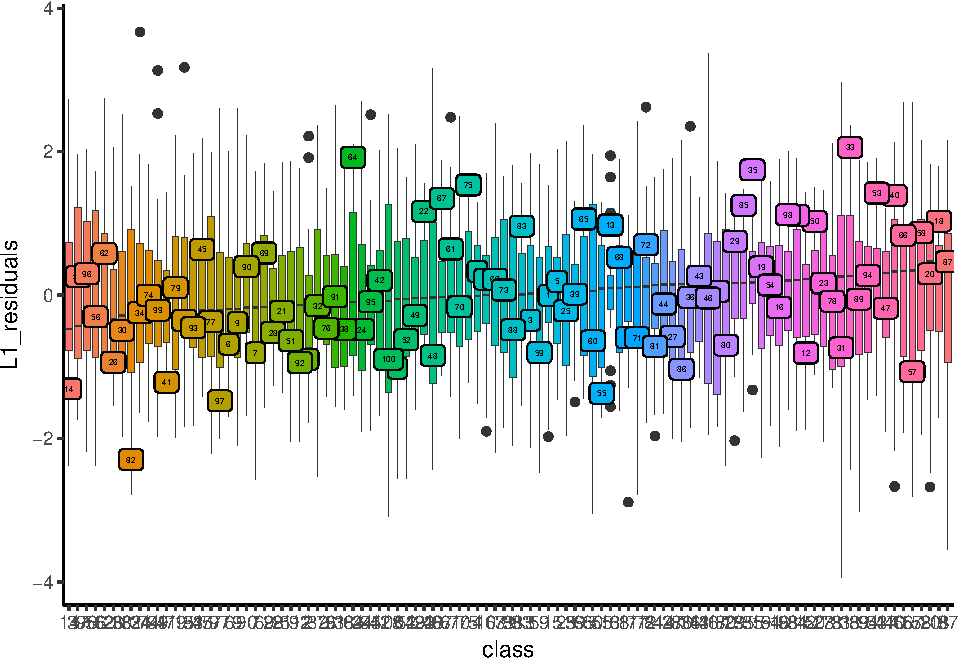
\includegraphics{Beck_HW_5_files/figure-latex/unnamed-chunk-2-1.pdf}

\section{Question 3}\label{question-3}

Examine the Level 1 residuals:

\subsection{Part A}\label{part-a}

Construct a Q-Q plot of the Level 1 residuals.

\begin{Shaded}
\begin{Highlighting}[]
\NormalTok{dat }\OperatorTok\StringTok{ }
\StringTok{  }\KeywordTok{ggplot}\NormalTok{(}\KeywordTok{aes}\NormalTok{(}\DataTypeTok{sample=}\NormalTok{L1_residuals)) }\OperatorTok{+}\StringTok{ }
\StringTok{  }\KeywordTok{stat_qq_band}\NormalTok{(}\DataTypeTok{fill =} \StringTok{"blue"}\NormalTok{, }\DataTypeTok{alpha =}\NormalTok{ .}\DecValTok{25}\NormalTok{) }\OperatorTok{+}
\StringTok{  }\KeywordTok{stat_qq_line}\NormalTok{() }\OperatorTok{+}\StringTok{ }
\StringTok{  }\KeywordTok{stat_qq_point}\NormalTok{() }\OperatorTok{+}
\StringTok{  }\KeywordTok{labs}\NormalTok{(}\DataTypeTok{x =} \StringTok{"Actual"}\NormalTok{, }\DataTypeTok{y =} \StringTok{"Theoretical"}\NormalTok{, }
       \DataTypeTok{title =} \StringTok{"Q-Q Plot of Studentized Residuals"}\NormalTok{) }\OperatorTok{+}
\StringTok{  }\KeywordTok{theme_classic}\NormalTok{()}
\end{Highlighting}
\end{Shaded}

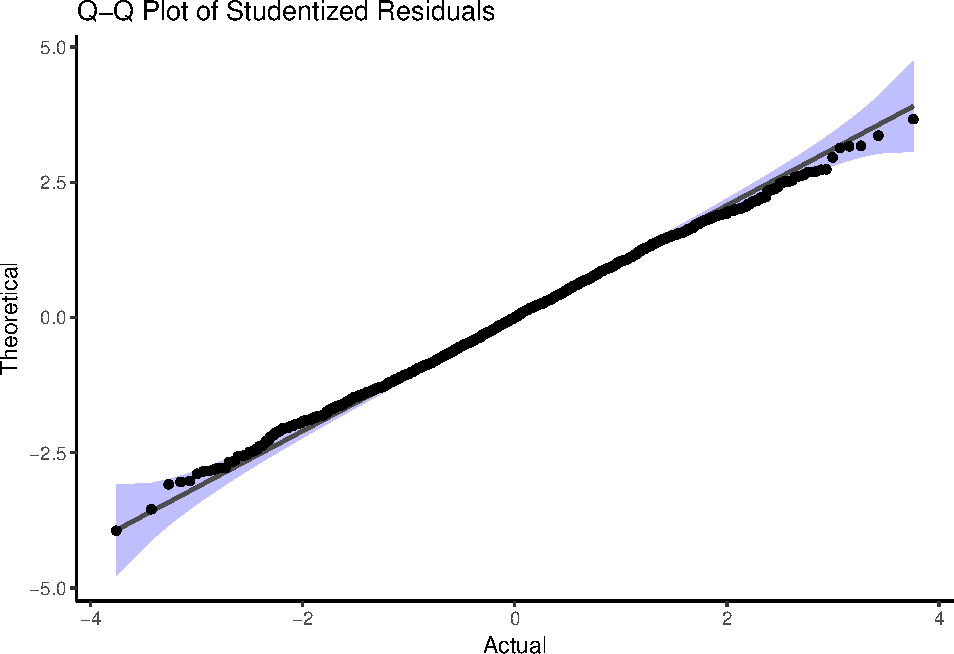
\includegraphics{Beck_HW_5_files/figure-latex/unnamed-chunk-3-1.pdf}

\subsection{Part B}\label{part-b}

Construct a histogram of the Level 1 residuals with a normal
distribution overlay.

\begin{Shaded}
\begin{Highlighting}[]
\NormalTok{dat }\OperatorTok
\StringTok{  }\KeywordTok{ggplot}\NormalTok{(}\KeywordTok{aes}\NormalTok{(}\DataTypeTok{x =}\NormalTok{ L1_residuals)) }\OperatorTok{+}
\StringTok{  }\KeywordTok{geom_density}\NormalTok{(}\DataTypeTok{fill =} \StringTok{"springgreen2"}\NormalTok{, }\DataTypeTok{alpha =}\NormalTok{ .}\DecValTok{6}\NormalTok{) }\OperatorTok{+}
\StringTok{  }\KeywordTok{stat_function}\NormalTok{(}\DataTypeTok{fun =}\NormalTok{ dnorm, }\DataTypeTok{size =} \FloatTok{1.25}\NormalTok{, }\DataTypeTok{color =} \StringTok{"darkgreen"}\NormalTok{, }\DataTypeTok{alpha =}\NormalTok{ .}\DecValTok{75}\NormalTok{,}
                \DataTypeTok{args =} \KeywordTok{list}\NormalTok{(}\DataTypeTok{mean =} \DecValTok{0}\NormalTok{, }\DataTypeTok{sd =}\DecValTok{1}\NormalTok{)) }\OperatorTok{+}
\StringTok{  }\KeywordTok{theme_classic}\NormalTok{()}
\end{Highlighting}
\end{Shaded}

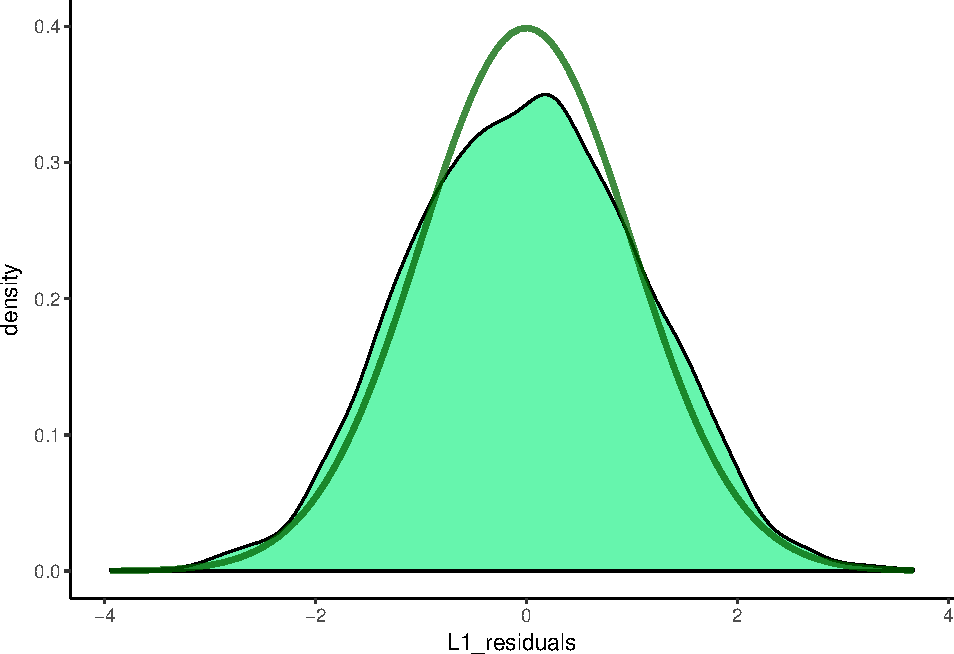
\includegraphics{Beck_HW_5_files/figure-latex/unnamed-chunk-4-1.pdf}

\subsection{Part C}\label{part-c}

Are the Level 1 residuals normally distributed? Yes, the level 1
residuals are normally distributed.

\subsection{Part D}\label{part-d}

Construct a scatterplot of the Level 1 residuals against the Level 1
fitted values. Comment on the assumption of homoscedasticity and what
that means for this unconditional model.

\begin{Shaded}
\begin{Highlighting}[]
\NormalTok{dat }\OperatorTok
\StringTok{  }\KeywordTok{ggplot}\NormalTok{(}\KeywordTok{aes}\NormalTok{(}\DataTypeTok{x =}\NormalTok{ .fitted, }\DataTypeTok{y =}\NormalTok{ L1_residuals)) }\OperatorTok{+}
\StringTok{  }\KeywordTok{geom_point}\NormalTok{() }\OperatorTok{+}
\StringTok{  }\KeywordTok{geom_smooth}\NormalTok{(}\DataTypeTok{method =} \StringTok{"lm"}\NormalTok{, }\DataTypeTok{se =}\NormalTok{ F) }\OperatorTok{+}
\StringTok{  }\KeywordTok{theme_classic}\NormalTok{()}
\end{Highlighting}
\end{Shaded}

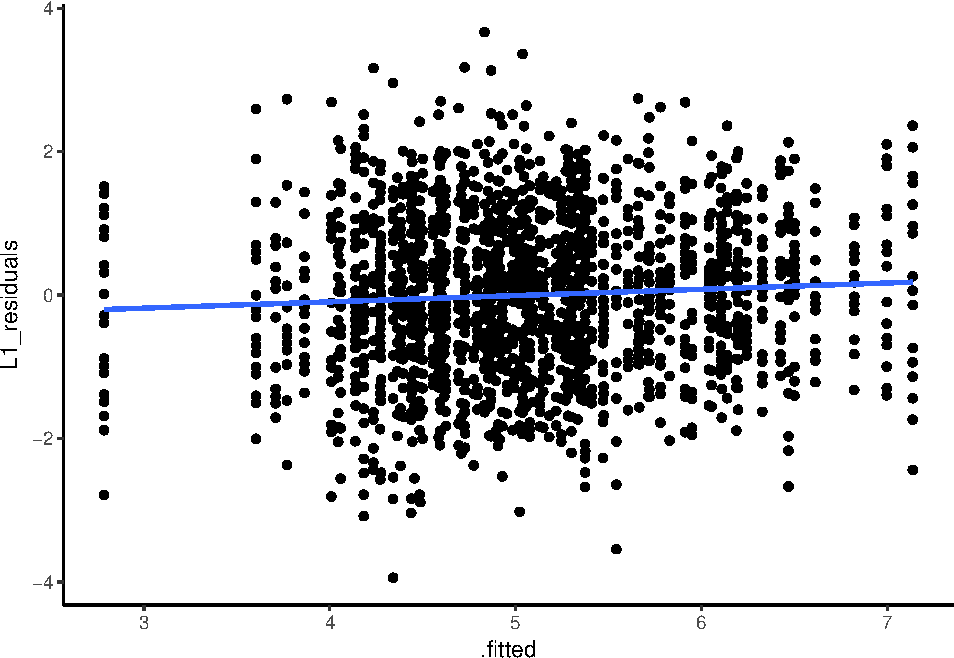
\includegraphics{Beck_HW_5_files/figure-latex/unnamed-chunk-5-1.pdf}

The plot of Level 1 residuals v. Level 1 fitted values suggests that we
meet the assumption of homoscedasticity. There is a very weak positive
relationship, but not strong enough to worry.

\section{Question 4}\label{question-4}

Now determine if Level 1 predictors should be added to the model.

\subsection{Part A}\label{part-a-1}

Correlate the Level 1 residuals with extraversion. Is there evidence
that this predictor should be included?

\begin{Shaded}
\begin{Highlighting}[]
\NormalTok{r <-}\StringTok{ }\NormalTok{dat }\OperatorTok\StringTok{ }\KeywordTok{select}\NormalTok{(extrav, sex12, .fitted, L1_residuals) }\OperatorTok\StringTok{ }\NormalTok{cor}

\NormalTok{r[}\KeywordTok{upper.tri}\NormalTok{(r, }\DataTypeTok{diag =}\NormalTok{ T)] <-}\StringTok{ }\OtherTok{NA}
\NormalTok{r <-}\StringTok{ }\NormalTok{r }\OperatorTok\StringTok{ }\KeywordTok{data.frame}\NormalTok{() }\OperatorTok\StringTok{ }\KeywordTok{mutate}\NormalTok{(}\DataTypeTok{v1 =} \KeywordTok{rownames}\NormalTok{(.)) }\OperatorTok\StringTok{ }\KeywordTok{select}\NormalTok{(v1, }\KeywordTok{everything}\NormalTok{())}

\KeywordTok{options}\NormalTok{(}\DataTypeTok{knitr.kable.NA =} \StringTok{''}\NormalTok{)}
\NormalTok{r }\OperatorTok
\StringTok{  }\KeywordTok{kable}\NormalTok{(., }\StringTok{"latex"}\NormalTok{, }\DataTypeTok{digits =} \DecValTok{2}\NormalTok{, }\DataTypeTok{booktabs =}\NormalTok{ T, }
        \DataTypeTok{col.names =} \KeywordTok{c}\NormalTok{(}\StringTok{""}\NormalTok{, }\StringTok{"extrav"}\NormalTok{, }\StringTok{"sex"}\NormalTok{, }\StringTok{"fitted"}\NormalTok{, }\StringTok{"L1 resid"}\NormalTok{))}
\end{Highlighting}
\end{Shaded}

\begin{tabular}{lrrrr}
\toprule
 & extrav & sex & fitted & L1 resid\\
\midrule
extrav &  &  &  & \\
sex12 & 0.09 &  &  & \\
.fitted & -0.01 & 0.26 &  & \\
L1\_residuals & 0.41 & 0.54 & 0.06 & \\
\bottomrule
\end{tabular}

Extraversion is moderately correlated with the level 1 residuals (r =
\(0.41\)), suggesting that it should be included in the model.

\subsection{Part B}\label{part-b-1}

Create a scatterplot showing the relationship between the Level 1
residuals and extraversion. Does there appear to be any need to model
nonlinearity?

\begin{Shaded}
\begin{Highlighting}[]
\NormalTok{dat }\OperatorTok
\StringTok{  }\KeywordTok{ggplot}\NormalTok{(}\KeywordTok{aes}\NormalTok{(}\DataTypeTok{x =}\NormalTok{ extrav, }\DataTypeTok{y =}\NormalTok{ L1_residuals)) }\OperatorTok{+}
\StringTok{  }\KeywordTok{geom_point}\NormalTok{() }\OperatorTok{+}
\StringTok{  }\KeywordTok{geom_smooth}\NormalTok{() }\OperatorTok{+}
\StringTok{  }\KeywordTok{theme_classic}\NormalTok{()}
\end{Highlighting}
\end{Shaded}

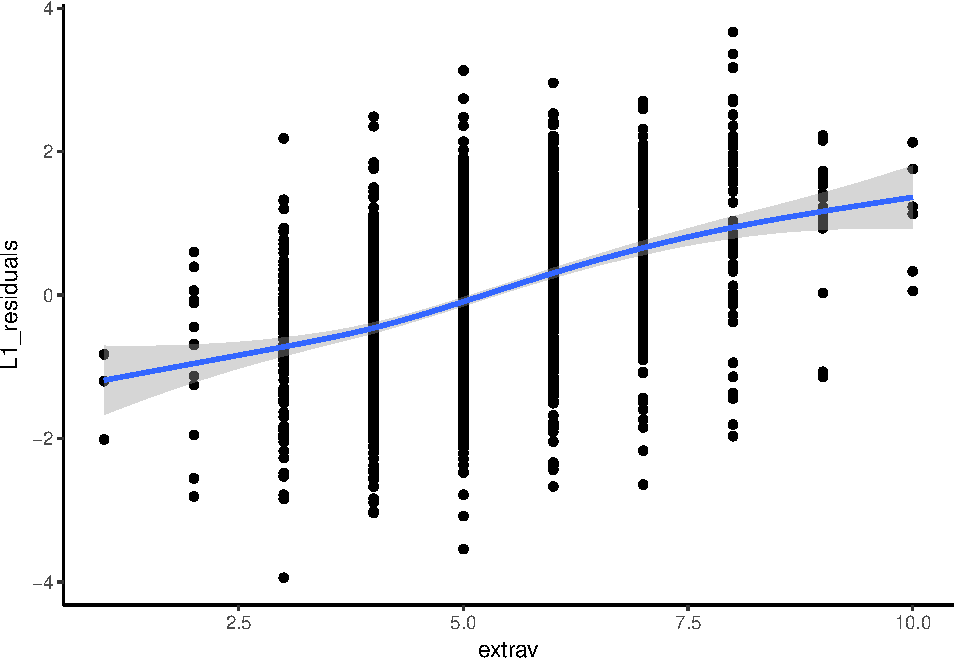
\includegraphics{Beck_HW_5_files/figure-latex/unnamed-chunk-7-1.pdf}

No, there is possibly a very small, non-linear effect, but the degree of
nonlinearity is very small.

\subsection{Part C}\label{part-c-1}

Correlate the Level 1 residuals with student sex. Is there evidence that
this predictor should be included? Sex is moderately to strongly
correlated with the level 1 residuals (\(r = 0.54\)), suggesting that it
should be included in the model.

\subsection{Part D}\label{part-d-1}

Should both predictors be included in the model? That is, do they appear
to be unique predictors?

Extraversion and sex are nearly uncorrelated (r = \(0.09\)), suggesting
that they do appear to be unique predictors.

\section{Question 5}\label{question-5}

Examine the Level 2 residuals:

\subsection{Part A}\label{part-a-2}

Create a classroom level data frame (call it Class\_Data) that contains
the Level 2 residuals (only intercept residuals are available so far;
name it R\_Intercept) and the grand-mean centered classroom means for
extraversion (name it Mean\_E\_GMC).

\begin{Shaded}
\begin{Highlighting}[]
\NormalTok{Class_Data <-}\StringTok{ }\NormalTok{dat }\OperatorTok
\StringTok{  }\KeywordTok{mutate}\NormalTok{(}\DataTypeTok{gmc =} \KeywordTok{mean}\NormalTok{(extrav, }\DataTypeTok{na.r =}\NormalTok{ T)) }\OperatorTok\StringTok{ }
\StringTok{  }\KeywordTok{group_by}\NormalTok{(class) }\OperatorTok\StringTok{ }
\StringTok{  }\KeywordTok{summarise}\NormalTok{(}\DataTypeTok{Mean_E_GMC =} \KeywordTok{mean}\NormalTok{(extrav, }\DataTypeTok{na.rm =}\NormalTok{ T)}\OperatorTok{/}\KeywordTok{unique}\NormalTok{(gmc)) }\OperatorTok
\StringTok{  }\KeywordTok{full_join}\NormalTok{(}\KeywordTok{unique}\NormalTok{(dat }\OperatorTok\StringTok{ }\KeywordTok{select}\NormalTok{(class, L2_residuals)))}
\end{Highlighting}
\end{Shaded}

\subsection{Part B}\label{part-b-2}

Construct a Q-Q plot of the Level 2 residuals

\begin{Shaded}
\begin{Highlighting}[]
\NormalTok{Class_Data }\OperatorTok\StringTok{ }
\StringTok{  }\KeywordTok{ggplot}\NormalTok{(}\KeywordTok{aes}\NormalTok{(}\DataTypeTok{sample=}\NormalTok{L2_residuals)) }\OperatorTok{+}\StringTok{ }
\StringTok{  }\KeywordTok{stat_qq_band}\NormalTok{(}\DataTypeTok{fill =} \StringTok{"blue"}\NormalTok{, }\DataTypeTok{alpha =}\NormalTok{ .}\DecValTok{25}\NormalTok{) }\OperatorTok{+}
\StringTok{  }\KeywordTok{stat_qq_line}\NormalTok{() }\OperatorTok{+}\StringTok{ }
\StringTok{  }\KeywordTok{stat_qq_point}\NormalTok{() }\OperatorTok{+}
\StringTok{  }\KeywordTok{labs}\NormalTok{(}\DataTypeTok{x =} \StringTok{"Actual"}\NormalTok{, }\DataTypeTok{y =} \StringTok{"Theoretical"}\NormalTok{, }
       \DataTypeTok{title =} \StringTok{"Q-Q Plot of Studentized Residuals"}\NormalTok{) }\OperatorTok{+}
\StringTok{  }\KeywordTok{theme_classic}\NormalTok{()}
\end{Highlighting}
\end{Shaded}

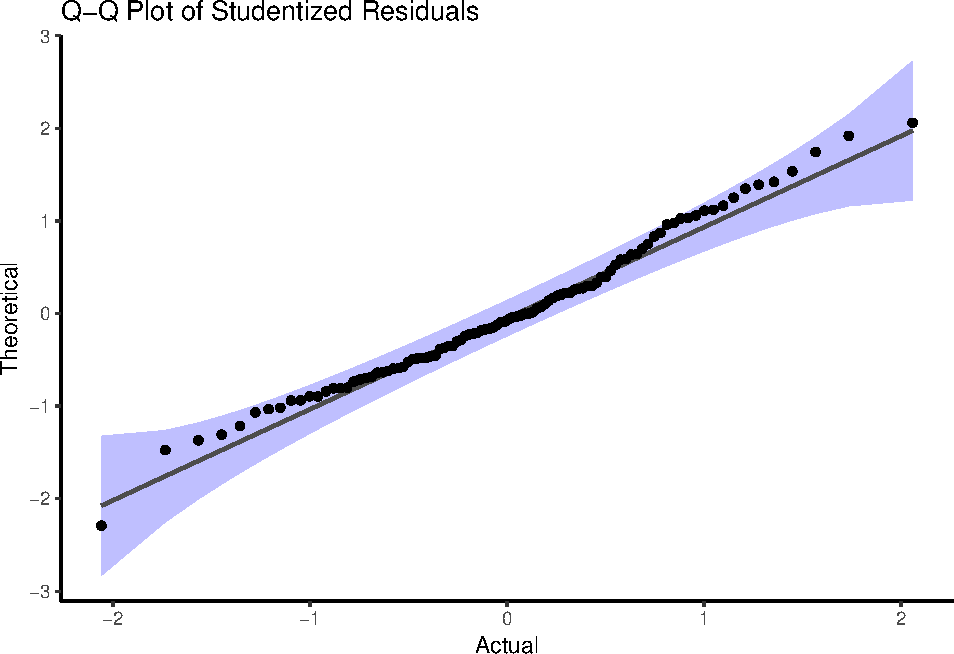
\includegraphics{Beck_HW_5_files/figure-latex/unnamed-chunk-9-1.pdf}

\subsection{Part C}\label{part-c-2}

Construct a histogram of the Level 2 residuals with a normal
distribution overlay.

\begin{Shaded}
\begin{Highlighting}[]
\NormalTok{Class_Data }\OperatorTok
\StringTok{  }\KeywordTok{ggplot}\NormalTok{(}\KeywordTok{aes}\NormalTok{(}\DataTypeTok{x =}\NormalTok{ L2_residuals)) }\OperatorTok{+}
\StringTok{  }\KeywordTok{geom_density}\NormalTok{(}\DataTypeTok{fill =} \StringTok{"springgreen2"}\NormalTok{, }\DataTypeTok{alpha =}\NormalTok{ .}\DecValTok{6}\NormalTok{) }\OperatorTok{+}
\StringTok{  }\KeywordTok{stat_function}\NormalTok{(}\DataTypeTok{fun =}\NormalTok{ dnorm, }\DataTypeTok{size =} \FloatTok{1.25}\NormalTok{, }\DataTypeTok{color =} \StringTok{"darkgreen"}\NormalTok{, }\DataTypeTok{alpha =}\NormalTok{ .}\DecValTok{75}\NormalTok{,}
                \DataTypeTok{args =} \KeywordTok{list}\NormalTok{(}\DataTypeTok{mean =} \DecValTok{0}\NormalTok{, }\DataTypeTok{sd =}\DecValTok{1}\NormalTok{)) }\OperatorTok{+}
\StringTok{  }\KeywordTok{theme_classic}\NormalTok{()}
\end{Highlighting}
\end{Shaded}

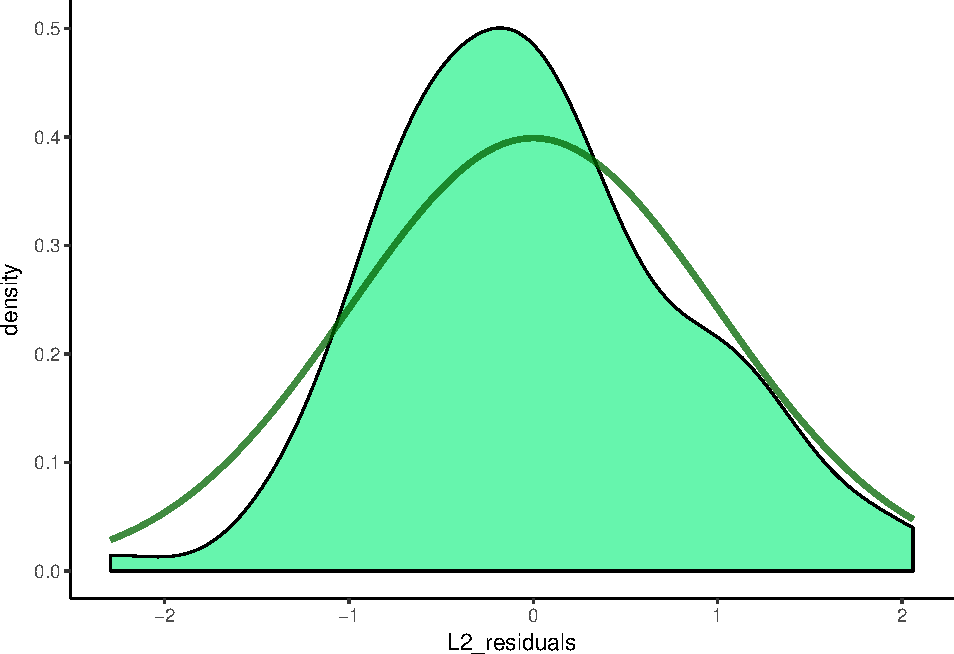
\includegraphics{Beck_HW_5_files/figure-latex/unnamed-chunk-10-1.pdf}

\subsection{Part D}\label{part-d-2}

Are the Level 2 residuals normally distributed? The Level 2 residuals do
not appear to be normally distributed.

\subsection{Part E}\label{part-e}

Correlate the Level 2 residuals with classroom mean extraversion. Is
there evidence that this predictor should be included in the Level 2
model?

\begin{Shaded}
\begin{Highlighting}[]
\NormalTok{r2 <-}\StringTok{ }\NormalTok{Class_Data }\OperatorTok\StringTok{ }\KeywordTok{summarize}\NormalTok{(}\DataTypeTok{r =} \KeywordTok{cor}\NormalTok{(Mean_E_GMC, L2_residuals))}
\end{Highlighting}
\end{Shaded}

Classroom mean extraversion is almost entirely uncorrellated
(\(r = -0.02\)) with the Level 2 resiudals.

\subsection{Part F}\label{part-f}

Create a scatterplot showing the relationship between the Level 2
residuals and classroom mean extraversion. Does there appear to be any
need to model nonlinearity at Level 2?

\begin{Shaded}
\begin{Highlighting}[]
\NormalTok{Class_Data }\OperatorTok
\StringTok{  }\KeywordTok{ggplot}\NormalTok{(}\KeywordTok{aes}\NormalTok{(}\DataTypeTok{x =}\NormalTok{ L2_residuals, }\DataTypeTok{y =}\NormalTok{ Mean_E_GMC)) }\OperatorTok{+}
\StringTok{  }\KeywordTok{geom_point}\NormalTok{() }\OperatorTok{+}
\StringTok{  }\KeywordTok{geom_smooth}\NormalTok{() }\OperatorTok{+}
\StringTok{  }\KeywordTok{theme_classic}\NormalTok{()}
\end{Highlighting}
\end{Shaded}

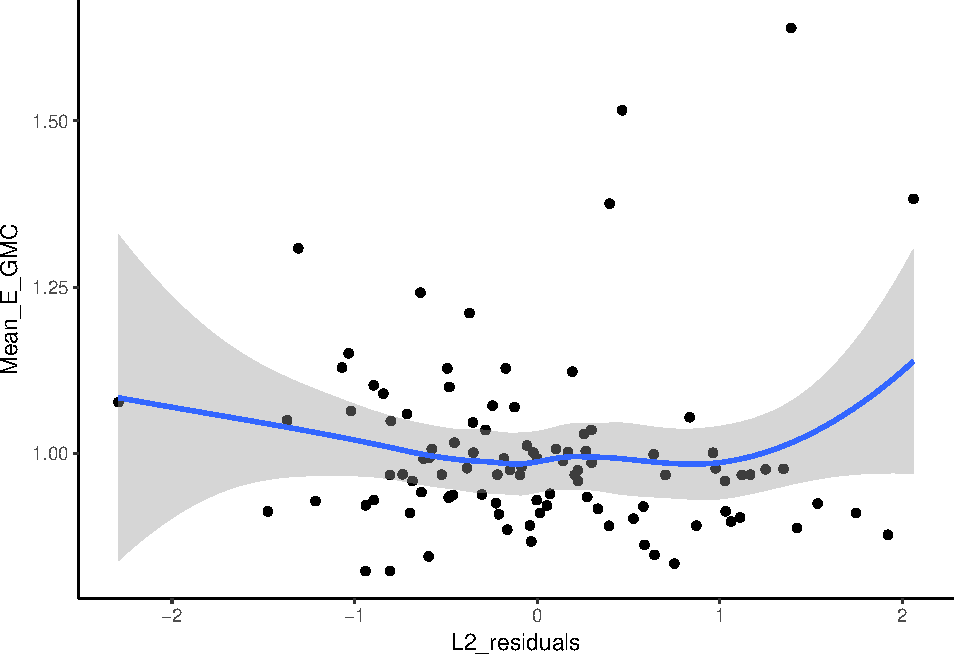
\includegraphics{Beck_HW_5_files/figure-latex/unnamed-chunk-12-1.pdf}

The relationship between classroom mean extraversion and the Level 2
residuals does appear to be slightly nonlinear.

\section{Question 6}\label{question-6}

\begin{enumerate}
\def\labelenumi{\arabic{enumi}.}
\setcounter{enumi}{5}
\tightlist
\item
  Fit a new model based on what you have discovered so far:\\
  To fit this model, you will need to create a new variable,
  Mean\_E\_GMC\_SQ, that is the square of Mean\_E\_GMC. Merge both
  variables into the original data frame, and fit the new model (call it
  Pop\_Fit\_3). Use the lme4 package so that you don't encounter
  convergence problems. Is there any evidence of curvilinearity at Level
  2?
\end{enumerate}

\begin{Shaded}
\begin{Highlighting}[]
\NormalTok{dat <-}\StringTok{ }\NormalTok{Class_Data }\OperatorTok\StringTok{ }\KeywordTok{mutate}\NormalTok{(}\DataTypeTok{Mean_E_GMC_SQ =}\NormalTok{ Mean_E_GMC}\OperatorTok{^}\DecValTok{2}\NormalTok{) }\OperatorTok
\StringTok{  }\KeywordTok{full_join}\NormalTok{(dat)}

\NormalTok{Pop_Fit_}\DecValTok{3}\NormalTok{ <-}\StringTok{ }\KeywordTok{lmer}\NormalTok{(popular }\OperatorTok{~}\StringTok{  }\NormalTok{extrav}\OperatorTok{*}\NormalTok{Mean_E_GMC }\OperatorTok{+}\StringTok{ }\NormalTok{extrav}\OperatorTok{*}\NormalTok{Mean_E_GMC_SQ }\OperatorTok{+}\StringTok{ }\NormalTok{sex}\OperatorTok{*}\NormalTok{Mean_E_GMC }\OperatorTok{+}\StringTok{ }
\StringTok{                    }\NormalTok{sex}\OperatorTok{*}\NormalTok{Mean_E_GMC_SQ }\OperatorTok{+}\StringTok{ }\NormalTok{(extrav }\OperatorTok{+}\StringTok{ }\NormalTok{sex}\OperatorTok{|}\NormalTok{class), }\DataTypeTok{data =}\NormalTok{ dat)}

\KeywordTok{table_fun}\NormalTok{(Pop_Fit_}\DecValTok{3}\NormalTok{)  }\OperatorTok
\StringTok{  }\KeywordTok{mutate}\NormalTok{(}\DataTypeTok{term =} \KeywordTok{str_replace_all}\NormalTok{(term, }\StringTok{"_"}\NormalTok{, }\StringTok{" "}\NormalTok{)) }\OperatorTok
\StringTok{  }\KeywordTok{select}\NormalTok{(}\OperatorTok{-}\NormalTok{type) }\OperatorTok
\StringTok{  }\KeywordTok{kable}\NormalTok{(., }\StringTok{"latex"}\NormalTok{, }\DataTypeTok{escape =}\NormalTok{ F, }\DataTypeTok{booktabs =}\NormalTok{ T,}
        \DataTypeTok{col.names =} \KeywordTok{c}\NormalTok{(}\StringTok{"Term"}\NormalTok{, }\KeywordTok{c}\NormalTok{(}\StringTok{"b"}\NormalTok{, }\StringTok{"CI"}\NormalTok{))) }\OperatorTok
\StringTok{  }\KeywordTok{add_header_above}\NormalTok{(}\KeywordTok{c}\NormalTok{(}\StringTok{" "}\NormalTok{ =}\StringTok{ }\DecValTok{1}\NormalTok{, }\StringTok{"Fit 3"}\NormalTok{)) }\OperatorTok
\StringTok{  }\KeywordTok{group_rows}\NormalTok{(}\StringTok{"Fixed"}\NormalTok{, }\DecValTok{1}\NormalTok{,}\DecValTok{9}\NormalTok{) }\OperatorTok
\StringTok{  }\KeywordTok{group_rows}\NormalTok{(}\StringTok{"Random"}\NormalTok{, }\DecValTok{10}\NormalTok{,}\DecValTok{12}\NormalTok{) }\OperatorTok
\StringTok{  }\KeywordTok{group_rows}\NormalTok{(}\StringTok{"Fixed"}\NormalTok{, }\DecValTok{13}\NormalTok{,}\DecValTok{14}\NormalTok{)}
\end{Highlighting}
\end{Shaded}

\begin{tabular}{lll}
\toprule
\multicolumn{1}{c}{ } & \multicolumn{1}{c}{Fit 3} \\
\cmidrule(l{2pt}r{2pt}){2-2}
Term & b & CI\\
\midrule
\addlinespace[0.3em]
\multicolumn{3}{l}{\textbf{Fixed}}\\
\hspace{1em}(Intercept) & 20.34 & [12.05, 26.86]\\
\hspace{1em}extrav & -1.41 & [-2.09, -0.32]\\
\hspace{1em}Mean E GMC & -26.12 & [-38.05, -9.88]\\
\hspace{1em}Mean E GMC SQ & 7.67 & [0.15, 13.56]\\
\hspace{1em}sexFemale & 0.49 & [-2.30, 4.74]\\
\hspace{1em}extrav:Mean E GMC & 2.66 & [0.56, 4.14]\\
\hspace{1em}extrav:Mean E GMC SQ & -0.79 & [-1.55, 0.20]\\
\hspace{1em}Mean E GMC:sexFemale & 0.99 & [-6.99, 6.15]\\
\hspace{1em}Mean E GMC SQ:sexFemale & -0.22 & [-2.59, 3.42]\\
\addlinespace[0.3em]
\multicolumn{3}{l}{\textbf{Random}}\\
\hspace{1em}$\tau {00}$ & 1.58 & [1.08, 2.19]\\
\hspace{1em}$\tau {11}$ & 0.02 & [0.01, 0.03]\\
\hspace{1em}$\tau {22}$ & 0.00 & [0.00, 0.02]\\
$R^2 m$ & 0.43 & \\
$R^2 c$ & 0.70 & \\
\bottomrule
\end{tabular}

There is no evidence of linearity at Level 2 (all t's \textless{} 1.6).

\section{Question 7}\label{question-7}

Fit a model that eliminates the squared terms in Level 2 (call it
Pop\_Fit\_4) and compare it to the full model. Are you justified in
eliminating the squared terms?

\begin{Shaded}
\begin{Highlighting}[]
\NormalTok{Pop_Fit_}\DecValTok{4}\NormalTok{ <-}\StringTok{ }\KeywordTok{lmer}\NormalTok{(popular }\OperatorTok{~}\StringTok{ }\NormalTok{extrav}\OperatorTok{*}\NormalTok{Mean_E_GMC }\OperatorTok{+}\StringTok{ }\NormalTok{sex}\OperatorTok{*}\NormalTok{Mean_E_GMC }\OperatorTok{+}\StringTok{ }\NormalTok{(extrav }\OperatorTok{+}\StringTok{ }\NormalTok{sex }\OperatorTok{|}\StringTok{ }\NormalTok{class), }\DataTypeTok{data =}\NormalTok{ dat)}

\KeywordTok{table_fun}\NormalTok{(Pop_Fit_}\DecValTok{4}\NormalTok{)  }\OperatorTok
\StringTok{  }\KeywordTok{mutate}\NormalTok{(}\DataTypeTok{term =} \KeywordTok{str_replace_all}\NormalTok{(term, }\StringTok{"_"}\NormalTok{, }\StringTok{" "}\NormalTok{)) }\OperatorTok
\StringTok{  }\KeywordTok{select}\NormalTok{(}\OperatorTok{-}\NormalTok{type) }\OperatorTok
\StringTok{  }\KeywordTok{kable}\NormalTok{(., }\StringTok{"latex"}\NormalTok{, }\DataTypeTok{escape =}\NormalTok{ F, }\DataTypeTok{booktabs =}\NormalTok{ T,}
        \DataTypeTok{col.names =} \KeywordTok{c}\NormalTok{(}\StringTok{"Term"}\NormalTok{, }\KeywordTok{c}\NormalTok{(}\StringTok{"b"}\NormalTok{, }\StringTok{"CI"}\NormalTok{))) }\OperatorTok
\StringTok{  }\KeywordTok{add_header_above}\NormalTok{(}\KeywordTok{c}\NormalTok{(}\StringTok{" "}\NormalTok{ =}\StringTok{ }\DecValTok{1}\NormalTok{, }\StringTok{"Fit 4"}\NormalTok{)) }\OperatorTok
\StringTok{  }\KeywordTok{group_rows}\NormalTok{(}\StringTok{"Fixed"}\NormalTok{, }\DecValTok{1}\NormalTok{,}\DecValTok{6}\NormalTok{) }\OperatorTok
\StringTok{  }\KeywordTok{group_rows}\NormalTok{(}\StringTok{"Random"}\NormalTok{, }\DecValTok{7}\NormalTok{,}\DecValTok{9}\NormalTok{) }\OperatorTok
\StringTok{  }\KeywordTok{group_rows}\NormalTok{(}\StringTok{"Fixed"}\NormalTok{, }\DecValTok{10}\NormalTok{,}\DecValTok{11}\NormalTok{)}
\end{Highlighting}
\end{Shaded}

\begin{tabular}{lll}
\toprule
\multicolumn{1}{c}{ } & \multicolumn{1}{c}{Fit 4} \\
\cmidrule(l{2pt}r{2pt}){2-2}
Term & b & CI\\
\midrule
\addlinespace[0.3em]
\multicolumn{3}{l}{\textbf{Fixed}}\\
\hspace{1em}(Intercept) & 10.84 & [8.75, 12.70]\\
\hspace{1em}extrav & -0.43 & [-0.68, -0.11]\\
\hspace{1em}Mean E GMC & -8.82 & [-10.75, -6.73]\\
\hspace{1em}sexFemale & 0.72 & [0.22, 1.08]\\
\hspace{1em}extrav:Mean E GMC & 0.88 & [0.56, 1.14]\\
\hspace{1em}Mean E GMC:sexFemale & 0.53 & [0.22, 1.01]\\
\addlinespace[0.3em]
\multicolumn{3}{l}{\textbf{Random}}\\
\hspace{1em}$\tau {00}$ & 1.59 & [0.86, 2.19]\\
\hspace{1em}$\tau {11}$ & 0.02 & [0.01, 0.03]\\
\hspace{1em}$\tau {22}$ & 0.00 & [0.00, 0.04]\\
$R^2 m$ & 0.41 & \\
$R^2 c$ & 0.69 & \\
\bottomrule
\end{tabular}

\begin{Shaded}
\begin{Highlighting}[]
\KeywordTok{anova}\NormalTok{(Pop_Fit_}\DecValTok{4}\NormalTok{, Pop_Fit_}\DecValTok{3}\NormalTok{)}
\end{Highlighting}
\end{Shaded}

Data: dat Models: Pop\_Fit\_4: popular \textasciitilde{} extrav *
Mean\_E\_GMC + sex * Mean\_E\_GMC + (extrav + Pop\_Fit\_4: sex
\textbar{} class) Pop\_Fit\_3: popular \textasciitilde{} extrav *
Mean\_E\_GMC + extrav * Mean\_E\_GMC\_SQ + sex * Pop\_Fit\_3:
Mean\_E\_GMC + sex * Mean\_E\_GMC\_SQ + (extrav + sex \textbar{} class)
Df AIC BIC logLik deviance Chisq Chi Df Pr(\textgreater{}Chisq)
Pop\_Fit\_4 13 4837.8 4910.6 -2405.9 4811.8\\
Pop\_Fit\_3 16 4841.2 4930.8 -2404.6 4809.2 2.6108 3 0.4556

Debatably, the model that includes the squared term not better than the
one that doesn't. I would drop it.

\section{Question 8}\label{question-8}

Using the simpler Pop\_Fit\_4 model, determine if either or both of the
slope variances at Level 2 can be set to 0.

\begin{Shaded}
\begin{Highlighting}[]
\NormalTok{Pop_Fit_4a <-}\StringTok{ }\KeywordTok{lmer}\NormalTok{(popular }\OperatorTok{~}\StringTok{ }\NormalTok{extrav}\OperatorTok{*}\NormalTok{Mean_E_GMC }\OperatorTok{+}\StringTok{ }\NormalTok{sex}\OperatorTok{*}\NormalTok{Mean_E_GMC }\OperatorTok{+}\StringTok{ }\NormalTok{(extrav }\OperatorTok{|}\StringTok{ }\NormalTok{class), }\DataTypeTok{data =}\NormalTok{ dat)}
\NormalTok{Pop_Fit_4b <-}\StringTok{ }\KeywordTok{lmer}\NormalTok{(popular }\OperatorTok{~}\StringTok{ }\NormalTok{extrav}\OperatorTok{*}\NormalTok{Mean_E_GMC }\OperatorTok{+}\StringTok{ }\NormalTok{sex}\OperatorTok{*}\NormalTok{Mean_E_GMC }\OperatorTok{+}\StringTok{ }\NormalTok{(sex }\OperatorTok{|}\StringTok{ }\NormalTok{class), }\DataTypeTok{data =}\NormalTok{ dat)}
\NormalTok{Pop_Fit_4c <-}\StringTok{ }\KeywordTok{lmer}\NormalTok{(popular }\OperatorTok{~}\StringTok{ }\NormalTok{extrav}\OperatorTok{*}\NormalTok{Mean_E_GMC }\OperatorTok{+}\StringTok{ }\NormalTok{sex}\OperatorTok{*}\NormalTok{Mean_E_GMC }\OperatorTok{+}\StringTok{ }\NormalTok{(}\DecValTok{1} \OperatorTok{|}\StringTok{ }\NormalTok{class), }\DataTypeTok{data =}\NormalTok{ dat)}

\NormalTok{f4a.tab <-}\StringTok{ }\KeywordTok{table_fun}\NormalTok{(Pop_Fit_4a)}
\NormalTok{f4b.tab <-}\StringTok{ }\KeywordTok{table_fun}\NormalTok{(Pop_Fit_4b)}
\NormalTok{f4c.tab <-}\StringTok{ }\KeywordTok{table_fun}\NormalTok{(Pop_Fit_4c)}

\NormalTok{f4a.tab }\OperatorTok\StringTok{ }\KeywordTok{mutate}\NormalTok{(}\DataTypeTok{model =} \StringTok{"Fit 4a"}\NormalTok{) }\OperatorTok
\StringTok{  }\KeywordTok{full_join}\NormalTok{(f4b.tab }\OperatorTok\StringTok{ }\KeywordTok{mutate}\NormalTok{(}\DataTypeTok{model =} \StringTok{"Fit 4b"}\NormalTok{)) }\OperatorTok
\StringTok{  }\KeywordTok{full_join}\NormalTok{(f4c.tab }\OperatorTok\StringTok{ }\KeywordTok{mutate}\NormalTok{(}\DataTypeTok{model =} \StringTok{"Fit 4c"}\NormalTok{))  }\OperatorTok
\StringTok{  }\KeywordTok{mutate}\NormalTok{(}\DataTypeTok{term =} \KeywordTok{str_replace_all}\NormalTok{(term, }\StringTok{"_"}\NormalTok{, }\StringTok{" "}\NormalTok{)) }\OperatorTok
\StringTok{  }\KeywordTok{gather}\NormalTok{(}\DataTypeTok{key =}\NormalTok{ est, }\DataTypeTok{value =}\NormalTok{ value, b, CI) }\OperatorTok
\StringTok{  }\KeywordTok{unite}\NormalTok{(tmp, model, est, }\DataTypeTok{sep =} \StringTok{"."}\NormalTok{) }\OperatorTok
\StringTok{  }\KeywordTok{mutate}\NormalTok{(}\DataTypeTok{type =} \KeywordTok{factor}\NormalTok{(type, }\DataTypeTok{levels =} \KeywordTok{c}\NormalTok{(}\StringTok{"Fixed Parts"}\NormalTok{, }\StringTok{"Random Parts"}\NormalTok{, }\StringTok{"Model Terms"}\NormalTok{))) }\OperatorTok
\StringTok{  }\KeywordTok{spread}\NormalTok{(}\DataTypeTok{key =}\NormalTok{ tmp, }\DataTypeTok{value =}\NormalTok{ value) }\OperatorTok
\StringTok{  }\KeywordTok{select}\NormalTok{(}\OperatorTok{-}\NormalTok{type) }\OperatorTok
\StringTok{  }\KeywordTok{kable}\NormalTok{(., }\StringTok{"latex"}\NormalTok{, }\DataTypeTok{escape =}\NormalTok{ F, }\DataTypeTok{booktabs =}\NormalTok{ T,}
        \DataTypeTok{col.names =} \KeywordTok{c}\NormalTok{(}\StringTok{"Term"}\NormalTok{, }\KeywordTok{rep}\NormalTok{(}\KeywordTok{c}\NormalTok{(}\StringTok{"b"}\NormalTok{, }\StringTok{"CI"}\NormalTok{), }\DataTypeTok{times =} \DecValTok{3}\NormalTok{))) }\OperatorTok
\StringTok{  }\KeywordTok{add_header_above}\NormalTok{(}\KeywordTok{c}\NormalTok{(}\StringTok{" "}\NormalTok{ =}\StringTok{ }\DecValTok{1}\NormalTok{, }\StringTok{"extrav RE"}\NormalTok{ =}\StringTok{ }\DecValTok{2}\NormalTok{, }\StringTok{"sex RE"}\NormalTok{ =}\StringTok{ }\DecValTok{2}\NormalTok{, }\StringTok{"No RE Slopes"}\NormalTok{ =}\StringTok{ }\DecValTok{2}\NormalTok{)) }\OperatorTok
\StringTok{  }\KeywordTok{group_rows}\NormalTok{(}\StringTok{"Fixed"}\NormalTok{, }\DecValTok{1}\NormalTok{,}\DecValTok{6}\NormalTok{) }\OperatorTok
\StringTok{  }\KeywordTok{group_rows}\NormalTok{(}\StringTok{"Random"}\NormalTok{, }\DecValTok{7}\NormalTok{,}\DecValTok{8}\NormalTok{) }\OperatorTok
\StringTok{  }\KeywordTok{group_rows}\NormalTok{(}\StringTok{"Fixed"}\NormalTok{, }\DecValTok{9}\NormalTok{,}\DecValTok{10}\NormalTok{)}
\end{Highlighting}
\end{Shaded}

\begin{tabular}{lllllll}
\toprule
\multicolumn{1}{c}{ } & \multicolumn{2}{c}{extrav RE} & \multicolumn{2}{c}{sex RE} & \multicolumn{2}{c}{No RE Slopes} \\
\cmidrule(l{2pt}r{2pt}){2-3} \cmidrule(l{2pt}r{2pt}){4-5} \cmidrule(l{2pt}r{2pt}){6-7}
Term & b & CI & b & CI & b & CI\\
\midrule
\addlinespace[0.3em]
\multicolumn{7}{l}{\textbf{Fixed}}\\
\hspace{1em}(Intercept) & 10.86 & [8.67, 13.60] & 10.96 & [7.51, 11.73] & 10.97 & [9.51, 12.28]\\
\hspace{1em}extrav & -0.43 & [-0.57, -0.22] & -0.43 & [-0.58, -0.14] & -0.43 & [-0.57, -0.25]\\
\hspace{1em}extrav:Mean E GMC & 0.88 & [0.69, 1.02] & 0.88 & [0.58, 1.05] & 0.88 & [0.69, 1.01]\\
\hspace{1em}Mean E GMC & -8.85 & [-11.55, -6.62] & -8.94 & [-9.72, -5.41] & -8.96 & [-10.07, -7.51]\\
\hspace{1em}Mean E GMC:sexFemale & 0.55 & [0.04, 1.12] & 0.47 & [-0.36, 0.99] & 0.47 & [0.05, 1.16]\\
\hspace{1em}sexFemale & 0.70 & [0.18, 1.18] & 0.78 & [0.22, 1.57] & 0.78 & [0.06, 1.25]\\
\addlinespace[0.3em]
\multicolumn{7}{l}{\textbf{Random}}\\
\hspace{1em}$\tau {00}$ & 1.60 & [1.23, 2.02] & 0.49 & [0.33, 0.62] & 0.46 & [0.39, 0.59]\\
\hspace{1em}$\tau {11}$ & 0.02 & [0.02, 0.03] & 0.00 & [0.00, 0.02] &  & \\
$R^2 c$ & 0.69 &  & 0.68 &  & 0.68 & \\
$R^2 m$ & 0.41 &  & 0.41 &  & 0.41 & \\
\bottomrule
\end{tabular}

\begin{Shaded}
\begin{Highlighting}[]
\KeywordTok{anova}\NormalTok{(Pop_Fit_}\DecValTok{4}\NormalTok{, Pop_Fit_4a, Pop_Fit_4b, Pop_Fit_4c)}
\end{Highlighting}
\end{Shaded}

Data: dat Models: Pop\_Fit\_4c: popular \textasciitilde{} extrav *
Mean\_E\_GMC + sex * Mean\_E\_GMC + (1 \textbar{} class) Pop\_Fit\_4a:
popular \textasciitilde{} extrav * Mean\_E\_GMC + sex * Mean\_E\_GMC +
(extrav \textbar{} Pop\_Fit\_4a: class) Pop\_Fit\_4b: popular
\textasciitilde{} extrav * Mean\_E\_GMC + sex * Mean\_E\_GMC + (sex
\textbar{} class) Pop\_Fit\_4: popular \textasciitilde{} extrav *
Mean\_E\_GMC + sex * Mean\_E\_GMC + (extrav + Pop\_Fit\_4: sex
\textbar{} class) Df AIC BIC logLik deviance Chisq Chi Df
Pr(\textgreater{}Chisq)\\
Pop\_Fit\_4c 8 4865.8 4910.6 -2424.9 4849.8\\
Pop\_Fit\_4a 10 4833.0 4889.0 -2406.5 4813.0 36.802 2 1.020e-08
\textbf{\emph{ Pop\_Fit\_4b 10 4869.1 4925.1 -2424.6 4849.1 0.000 0 1\\
Pop\_Fit\_4 13 4837.8 4910.6 -2405.9 4811.8 37.315 3 3.947e-08 }} ---
Signif. codes: 0 `\emph{\textbf{' 0.001 '}' 0.01 '}' 0.05 `.' 0.1 `' 1

\subsection{Part A}\label{part-a-3}

Eliminate the random effect for extrav (call this model Pop\_Fit\_5). Is
this model indistinguishable from Pop\_Fit\_4?

\begin{Shaded}
\begin{Highlighting}[]
\NormalTok{Pop_Fit_}\DecValTok{5}\NormalTok{ <-}\StringTok{ }\KeywordTok{lmer}\NormalTok{(popular }\OperatorTok{~}\StringTok{ }\NormalTok{extrav}\OperatorTok{*}\NormalTok{Mean_E_GMC }\OperatorTok{+}\StringTok{ }\NormalTok{sex}\OperatorTok{*}\NormalTok{Mean_E_GMC }\OperatorTok{+}\StringTok{ }\NormalTok{(sex }\OperatorTok{|}\StringTok{ }\NormalTok{class), }\DataTypeTok{data =}\NormalTok{ dat)}

\KeywordTok{table_fun}\NormalTok{(Pop_Fit_}\DecValTok{5}\NormalTok{)  }\OperatorTok
\StringTok{  }\KeywordTok{mutate}\NormalTok{(}\DataTypeTok{term =} \KeywordTok{str_replace_all}\NormalTok{(term, }\StringTok{"_"}\NormalTok{, }\StringTok{" "}\NormalTok{)) }\OperatorTok
\StringTok{  }\KeywordTok{select}\NormalTok{(}\OperatorTok{-}\NormalTok{type) }\OperatorTok
\StringTok{  }\KeywordTok{kable}\NormalTok{(., }\StringTok{"latex"}\NormalTok{, }\DataTypeTok{escape =}\NormalTok{ F, }\DataTypeTok{booktabs =}\NormalTok{ T,}
        \DataTypeTok{col.names =} \KeywordTok{c}\NormalTok{(}\StringTok{"Term"}\NormalTok{, }\KeywordTok{c}\NormalTok{(}\StringTok{"b"}\NormalTok{, }\StringTok{"CI"}\NormalTok{))) }\OperatorTok
\StringTok{  }\KeywordTok{add_header_above}\NormalTok{(}\KeywordTok{c}\NormalTok{(}\StringTok{" "}\NormalTok{ =}\StringTok{ }\DecValTok{1}\NormalTok{, }\StringTok{"Fit 5"}\NormalTok{)) }\OperatorTok
\StringTok{  }\KeywordTok{group_rows}\NormalTok{(}\StringTok{"Fixed"}\NormalTok{, }\DecValTok{1}\NormalTok{,}\DecValTok{6}\NormalTok{) }\OperatorTok
\StringTok{  }\KeywordTok{group_rows}\NormalTok{(}\StringTok{"Random"}\NormalTok{, }\DecValTok{7}\NormalTok{,}\DecValTok{8}\NormalTok{) }\OperatorTok
\StringTok{  }\KeywordTok{group_rows}\NormalTok{(}\StringTok{"Fixed"}\NormalTok{, }\DecValTok{9}\NormalTok{,}\DecValTok{10}\NormalTok{)}
\end{Highlighting}
\end{Shaded}

\begin{tabular}{lll}
\toprule
\multicolumn{1}{c}{ } & \multicolumn{1}{c}{Fit 5} \\
\cmidrule(l{2pt}r{2pt}){2-2}
Term & b & CI\\
\midrule
\addlinespace[0.3em]
\multicolumn{3}{l}{\textbf{Fixed}}\\
\hspace{1em}(Intercept) & 10.96 & [9.75, 11.81]\\
\hspace{1em}extrav & -0.43 & [-0.60, -0.20]\\
\hspace{1em}Mean E GMC & -8.94 & [-9.62, -7.52]\\
\hspace{1em}sexFemale & 0.78 & [0.15, 1.53]\\
\hspace{1em}extrav:Mean E GMC & 0.88 & [0.62, 1.05]\\
\hspace{1em}Mean E GMC:sexFemale & 0.47 & [-0.23, 1.15]\\
\addlinespace[0.3em]
\multicolumn{3}{l}{\textbf{Random}}\\
\hspace{1em}$\tau {00}$ & 0.49 & [0.34, 0.66]\\
\hspace{1em}$\tau {11}$ & 0.00 & [0.00, 0.05]\\
$R^2 m$ & 0.41 & \\
$R^2 c$ & 0.68 & \\
\bottomrule
\end{tabular}

\begin{Shaded}
\begin{Highlighting}[]
\KeywordTok{anova}\NormalTok{(Pop_Fit_}\DecValTok{4}\NormalTok{, Pop_Fit_}\DecValTok{5}\NormalTok{)}
\end{Highlighting}
\end{Shaded}

Data: dat Models: Pop\_Fit\_5: popular \textasciitilde{} extrav *
Mean\_E\_GMC + sex * Mean\_E\_GMC + (sex \textbar{} class) Pop\_Fit\_4:
popular \textasciitilde{} extrav * Mean\_E\_GMC + sex * Mean\_E\_GMC +
(extrav + Pop\_Fit\_4: sex \textbar{} class) Df AIC BIC logLik deviance
Chisq Chi Df Pr(\textgreater{}Chisq)\\
Pop\_Fit\_5 10 4869.1 4925.1 -2424.6 4849.1\\
Pop\_Fit\_4 13 4837.8 4910.6 -2405.9 4811.8 37.315 3 3.947e-08 *** ---
Signif. codes: 0 `\emph{\textbf{' 0.001 '}' 0.01 '}' 0.05 `.' 0.1 `' 1

This model is distinguishable from the model from question 4 --
eliminating the extraversion random slope improves model fit.

\subsection{Part B}\label{part-b-3}

Eliminate the random effect for sex (call this model Pop\_Fit\_6). Is
this model indistinguishable from Pop\_Fit\_4?

\begin{Shaded}
\begin{Highlighting}[]
\NormalTok{Pop_Fit_}\DecValTok{6}\NormalTok{ <-}\StringTok{ }\KeywordTok{lmer}\NormalTok{(popular }\OperatorTok{~}\StringTok{ }\NormalTok{extrav}\OperatorTok{*}\NormalTok{Mean_E_GMC }\OperatorTok{+}\StringTok{ }\NormalTok{sex}\OperatorTok{*}\NormalTok{Mean_E_GMC }\OperatorTok{+}\StringTok{ }\NormalTok{(extrav }\OperatorTok{|}\StringTok{ }\NormalTok{class), }\DataTypeTok{data =}\NormalTok{ dat)}

\KeywordTok{table_fun}\NormalTok{(Pop_Fit_}\DecValTok{6}\NormalTok{)  }\OperatorTok
\StringTok{  }\KeywordTok{mutate}\NormalTok{(}\DataTypeTok{term =} \KeywordTok{str_replace_all}\NormalTok{(term, }\StringTok{"_"}\NormalTok{, }\StringTok{" "}\NormalTok{)) }\OperatorTok
\StringTok{  }\KeywordTok{select}\NormalTok{(}\OperatorTok{-}\NormalTok{type) }\OperatorTok
\StringTok{  }\KeywordTok{kable}\NormalTok{(., }\StringTok{"latex"}\NormalTok{, }\DataTypeTok{escape =}\NormalTok{ F, }\DataTypeTok{booktabs =}\NormalTok{ T,}
        \DataTypeTok{col.names =} \KeywordTok{c}\NormalTok{(}\StringTok{"Term"}\NormalTok{, }\KeywordTok{c}\NormalTok{(}\StringTok{"b"}\NormalTok{, }\StringTok{"CI"}\NormalTok{))) }\OperatorTok
\StringTok{  }\KeywordTok{add_header_above}\NormalTok{(}\KeywordTok{c}\NormalTok{(}\StringTok{" "}\NormalTok{ =}\StringTok{ }\DecValTok{1}\NormalTok{, }\StringTok{"Fit 6"}\NormalTok{)) }\OperatorTok
\StringTok{  }\KeywordTok{group_rows}\NormalTok{(}\StringTok{"Fixed"}\NormalTok{, }\DecValTok{1}\NormalTok{,}\DecValTok{6}\NormalTok{) }\OperatorTok
\StringTok{  }\KeywordTok{group_rows}\NormalTok{(}\StringTok{"Random"}\NormalTok{, }\DecValTok{7}\NormalTok{,}\DecValTok{8}\NormalTok{) }\OperatorTok
\StringTok{  }\KeywordTok{group_rows}\NormalTok{(}\StringTok{"Fixed"}\NormalTok{, }\DecValTok{9}\NormalTok{,}\DecValTok{10}\NormalTok{)}
\end{Highlighting}
\end{Shaded}

\begin{tabular}{lll}
\toprule
\multicolumn{1}{c}{ } & \multicolumn{1}{c}{Fit 6} \\
\cmidrule(l{2pt}r{2pt}){2-2}
Term & b & CI\\
\midrule
\addlinespace[0.3em]
\multicolumn{3}{l}{\textbf{Fixed}}\\
\hspace{1em}(Intercept) & 10.86 & [8.71, 12.03]\\
\hspace{1em}extrav & -0.43 & [-0.56, -0.23]\\
\hspace{1em}Mean E GMC & -8.85 & [-10.05, -6.60]\\
\hspace{1em}sexFemale & 0.70 & [0.02, 1.53]\\
\hspace{1em}extrav:Mean E GMC & 0.88 & [0.68, 1.00]\\
\hspace{1em}Mean E GMC:sexFemale & 0.55 & [-0.29, 1.21]\\
\addlinespace[0.3em]
\multicolumn{3}{l}{\textbf{Random}}\\
\hspace{1em}$\tau {00}$ & 1.60 & [1.29, 1.94]\\
\hspace{1em}$\tau {11}$ & 0.02 & [0.01, 0.03]\\
$R^2 m$ & 0.41 & \\
$R^2 c$ & 0.69 & \\
\bottomrule
\end{tabular}

\begin{Shaded}
\begin{Highlighting}[]
\KeywordTok{anova}\NormalTok{(Pop_Fit_}\DecValTok{4}\NormalTok{, Pop_Fit_}\DecValTok{6}\NormalTok{)}
\end{Highlighting}
\end{Shaded}

Data: dat Models: Pop\_Fit\_6: popular \textasciitilde{} extrav *
Mean\_E\_GMC + sex * Mean\_E\_GMC + (extrav \textbar{} Pop\_Fit\_6:
class) Pop\_Fit\_4: popular \textasciitilde{} extrav * Mean\_E\_GMC +
sex * Mean\_E\_GMC + (extrav + Pop\_Fit\_4: sex \textbar{} class) Df AIC
BIC logLik deviance Chisq Chi Df Pr(\textgreater{}Chisq) Pop\_Fit\_6 10
4833.0 4889.0 -2406.5 4813.0\\
Pop\_Fit\_4 13 4837.8 4910.6 -2405.9 4811.8 1.247 3 0.7418

Yes, the model that does not include the random slope for sex is
indistinguishable from one that does.

\subsection{Part C}\label{part-c-3}

Finally, eliminate them both (call this Pop\_Fit\_7) and compare it to
Pop\_Fit\_4. Which simpler model is justified?

\begin{Shaded}
\begin{Highlighting}[]
\NormalTok{Pop_Fit_}\DecValTok{7}\NormalTok{ <-}\StringTok{ }\KeywordTok{lmer}\NormalTok{(popular }\OperatorTok{~}\StringTok{ }\NormalTok{extrav}\OperatorTok{*}\NormalTok{Mean_E_GMC }\OperatorTok{+}\StringTok{ }\NormalTok{sex}\OperatorTok{*}\NormalTok{Mean_E_GMC }\OperatorTok{+}\StringTok{ }\NormalTok{(}\DecValTok{1} \OperatorTok{|}\StringTok{ }\NormalTok{class), }\DataTypeTok{data =}\NormalTok{ dat)}

\KeywordTok{table_fun}\NormalTok{(Pop_Fit_}\DecValTok{7}\NormalTok{) }\OperatorTok
\StringTok{  }\KeywordTok{mutate}\NormalTok{(}\DataTypeTok{term =} \KeywordTok{str_replace_all}\NormalTok{(term, }\StringTok{"_"}\NormalTok{, }\StringTok{" "}\NormalTok{)) }\OperatorTok
\StringTok{  }\KeywordTok{select}\NormalTok{(}\OperatorTok{-}\NormalTok{type) }\OperatorTok
\StringTok{  }\KeywordTok{kable}\NormalTok{(., }\StringTok{"latex"}\NormalTok{, }\DataTypeTok{escape =}\NormalTok{ F, }\DataTypeTok{booktabs =}\NormalTok{ T,}
        \DataTypeTok{col.names =} \KeywordTok{c}\NormalTok{(}\StringTok{"Term"}\NormalTok{, }\KeywordTok{c}\NormalTok{(}\StringTok{"b"}\NormalTok{, }\StringTok{"CI"}\NormalTok{))) }\OperatorTok
\StringTok{  }\KeywordTok{add_header_above}\NormalTok{(}\KeywordTok{c}\NormalTok{(}\StringTok{" "}\NormalTok{ =}\StringTok{ }\DecValTok{1}\NormalTok{, }\StringTok{"Fit 7"}\NormalTok{)) }\OperatorTok
\StringTok{  }\KeywordTok{group_rows}\NormalTok{(}\StringTok{"Fixed"}\NormalTok{, }\DecValTok{1}\NormalTok{,}\DecValTok{6}\NormalTok{) }\OperatorTok
\StringTok{  }\KeywordTok{group_rows}\NormalTok{(}\StringTok{"Random"}\NormalTok{, }\DecValTok{7}\NormalTok{,}\DecValTok{7}\NormalTok{) }\OperatorTok
\StringTok{  }\KeywordTok{group_rows}\NormalTok{(}\StringTok{"Fixed"}\NormalTok{, }\DecValTok{8}\NormalTok{,}\DecValTok{9}\NormalTok{)}
\end{Highlighting}
\end{Shaded}

\begin{tabular}{lll}
\toprule
\multicolumn{1}{c}{ } & \multicolumn{1}{c}{Fit 7} \\
\cmidrule(l{2pt}r{2pt}){2-2}
Term & b & CI\\
\midrule
\addlinespace[0.3em]
\multicolumn{3}{l}{\textbf{Fixed}}\\
\hspace{1em}(Intercept) & 10.97 & [8.75, 12.01]\\
\hspace{1em}extrav & -0.43 & [-0.66, -0.23]\\
\hspace{1em}Mean E GMC & -8.96 & [-10.02, -6.71]\\
\hspace{1em}sexFemale & 0.78 & [0.24, 1.48]\\
\hspace{1em}extrav:Mean E GMC & 0.88 & [0.69, 1.11]\\
\hspace{1em}Mean E GMC:sexFemale & 0.47 & [-0.23, 1.01]\\
\addlinespace[0.3em]
\multicolumn{3}{l}{\textbf{Random}}\\
\hspace{1em}$\tau {00}$ & 0.46 & [0.43, 0.60]\\
$R^2 m$ & 0.41 & \\
$R^2 c$ & 0.68 & \\
\bottomrule
\end{tabular}

\begin{Shaded}
\begin{Highlighting}[]
\KeywordTok{anova}\NormalTok{(Pop_Fit_}\DecValTok{4}\NormalTok{, Pop_Fit_}\DecValTok{7}\NormalTok{)}
\end{Highlighting}
\end{Shaded}

\begin{verbatim}
## Data: dat
## Models:
## Pop_Fit_7: popular ~ extrav * Mean_E_GMC + sex * Mean_E_GMC + (1 | class)
## Pop_Fit_4: popular ~ extrav * Mean_E_GMC + sex * Mean_E_GMC + (extrav + 
## Pop_Fit_4:     sex | class)
##           Df    AIC    BIC  logLik deviance  Chisq Chi Df Pr(>Chisq)    
## Pop_Fit_7  8 4865.8 4910.6 -2424.9   4849.8                             
## Pop_Fit_4 13 4837.8 4910.6 -2405.9   4811.8 38.049      5  3.689e-07 ***
## ---
## Signif. codes:  0 '***' 0.001 '**' 0.01 '*' 0.05 '.' 0.1 ' ' 1
\end{verbatim}

\begin{Shaded}
\begin{Highlighting}[]
\KeywordTok{anova}\NormalTok{(Pop_Fit_}\DecValTok{5}\NormalTok{, Pop_Fit_}\DecValTok{7}\NormalTok{)}
\end{Highlighting}
\end{Shaded}

\begin{verbatim}
## Data: dat
## Models:
## Pop_Fit_7: popular ~ extrav * Mean_E_GMC + sex * Mean_E_GMC + (1 | class)
## Pop_Fit_5: popular ~ extrav * Mean_E_GMC + sex * Mean_E_GMC + (sex | class)
##           Df    AIC    BIC  logLik deviance  Chisq Chi Df Pr(>Chisq)
## Pop_Fit_7  8 4865.8 4910.6 -2424.9   4849.8                         
## Pop_Fit_5 10 4869.1 4925.1 -2424.6   4849.1 0.7339      2     0.6928
\end{verbatim}

The simplest model with no random slopes is best because it is better
than a model that includes both but not better than one that includes
only sex.

\section{Question 9}\label{question-9}

Use the simplest model justified from the previous question.

\subsection{Part A}\label{part-a-4}

Retest the Level 1 homogeneity assumption. Is there any improvement
compared to what was found for Question 1?

\begin{Shaded}
\begin{Highlighting}[]
\NormalTok{Pop_Fit_}\FloatTok{7.}\NormalTok{lme <-}\StringTok{ }\KeywordTok{lme}\NormalTok{(popular }\OperatorTok{~}\StringTok{ }\NormalTok{extrav}\OperatorTok{*}\NormalTok{Mean_E_GMC }\OperatorTok{+}\StringTok{ }\NormalTok{sex}\OperatorTok{*}\NormalTok{Mean_E_GMC, }\DataTypeTok{random =} \OperatorTok{~}\StringTok{ }\DecValTok{1}\OperatorTok{|}\NormalTok{class, }\DataTypeTok{data =}\NormalTok{ dat)}
\NormalTok{Pop_Fit_}\FloatTok{7.}\NormalTok{a <-}\StringTok{ }\KeywordTok{lme}\NormalTok{(popular }\OperatorTok{~}\StringTok{ }\NormalTok{extrav}\OperatorTok{*}\NormalTok{Mean_E_GMC }\OperatorTok{+}\StringTok{ }\NormalTok{sex}\OperatorTok{*}\NormalTok{Mean_E_GMC, }\DataTypeTok{random =} \OperatorTok{~}\StringTok{ }\DecValTok{1}\OperatorTok{|}\NormalTok{class, }
                   \DataTypeTok{data =}\NormalTok{ dat, }\KeywordTok{varIdent}\NormalTok{(}\DataTypeTok{form =} \OperatorTok{~}\StringTok{ }\DecValTok{1} \OperatorTok{|}\StringTok{ }\NormalTok{class))}

\KeywordTok{anova}\NormalTok{(Pop_Fit_}\FloatTok{7.}\NormalTok{lme, Pop_Fit_}\FloatTok{7.}\NormalTok{a)}
\end{Highlighting}
\end{Shaded}

\begin{verbatim}
##               Model  df      AIC      BIC    logLik   Test  L.Ratio
## Pop_Fit_7.lme     1   8 4882.758 4927.541 -2433.379                
## Pop_Fit_7.a       2 107 4963.523 5562.499 -2374.762 1 vs 2 117.2343
##               p-value
## Pop_Fit_7.lme        
## Pop_Fit_7.a    0.1019
\end{verbatim}

In this case, we meet the homogeneity of variance assumption. The model
that fits unique variances is not better than one that does not.

\subsection{Part B}\label{part-b-4}

Check the multivariate normality assumption for the residuals at Level 2
using Mahalanobis distance. Are the residuals multivariate normal?

\begin{Shaded}
\begin{Highlighting}[]
\NormalTok{L2_residuals <-}\StringTok{ }\KeywordTok{ranef}\NormalTok{(Pop_Fit_}\DecValTok{7}\NormalTok{)[[}\DecValTok{1}\NormalTok{]]}
\NormalTok{MD.v <-}\StringTok{ }\KeywordTok{mahalanobis}\NormalTok{(L2_residuals, }\KeywordTok{colMeans}\NormalTok{(L2_residuals), }\KeywordTok{cov}\NormalTok{(L2_residuals))}

\NormalTok{MD.df <-}\StringTok{ }\NormalTok{MD.v }\OperatorTok\StringTok{ }\NormalTok{data.frame }\OperatorTok\StringTok{ }\KeywordTok{setNames}\NormalTok{(}\StringTok{"MD"}\NormalTok{) }\OperatorTok\StringTok{ }\KeywordTok{mutate}\NormalTok{(}\DataTypeTok{class =} \KeywordTok{names}\NormalTok{(MD.v)) }

\NormalTok{MD.df }\OperatorTok\StringTok{ }
\StringTok{  }\KeywordTok{ggplot}\NormalTok{(}\KeywordTok{aes}\NormalTok{(}\DataTypeTok{sample =}\NormalTok{ MD)) }\OperatorTok{+}
\StringTok{  }\KeywordTok{stat_qq_band}\NormalTok{(}\DataTypeTok{distribution =} \StringTok{"chisq"}\NormalTok{, }\DataTypeTok{dparams =} \KeywordTok{list}\NormalTok{(}\DataTypeTok{df =} \DecValTok{4}\NormalTok{)) }\OperatorTok{+}\StringTok{ }
\StringTok{  }\KeywordTok{stat_qq_line}\NormalTok{(}\DataTypeTok{distribution =} \StringTok{"chisq"}\NormalTok{, }\DataTypeTok{dparams =} \KeywordTok{list}\NormalTok{(}\DataTypeTok{df =} \DecValTok{4}\NormalTok{)) }\OperatorTok{+}\StringTok{ }
\StringTok{  }\KeywordTok{stat_qq_point}\NormalTok{(}\DataTypeTok{distribution =} \StringTok{"chisq"}\NormalTok{, }\DataTypeTok{dparams =} \KeywordTok{list}\NormalTok{(}\DataTypeTok{df =} \DecValTok{4}\NormalTok{)) }\OperatorTok{+}
\StringTok{  }\KeywordTok{theme_classic}\NormalTok{()}
\end{Highlighting}
\end{Shaded}

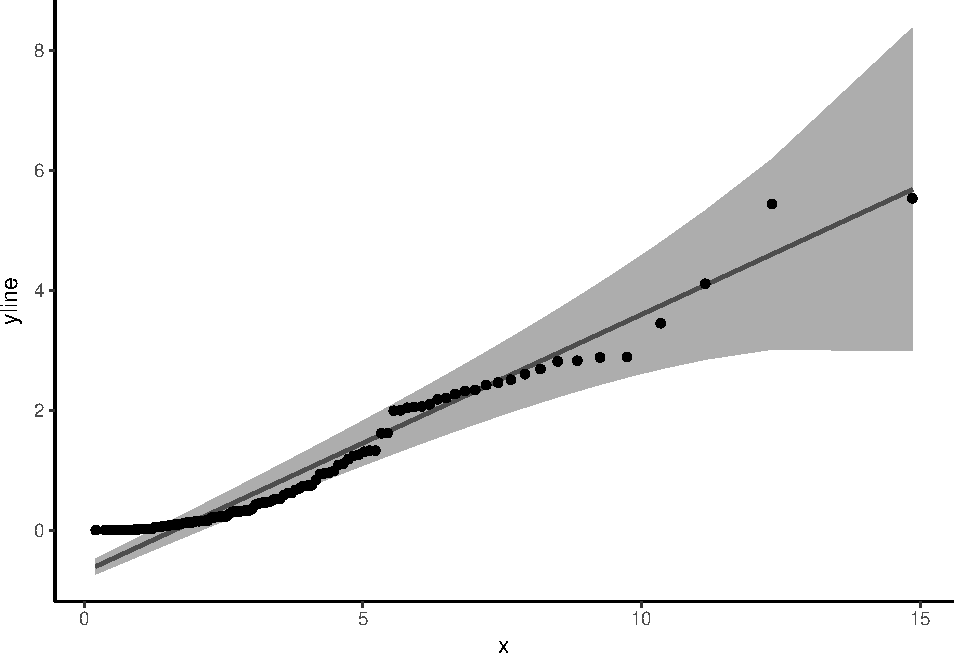
\includegraphics{Beck_HW_5_files/figure-latex/unnamed-chunk-20-1.pdf}

The residuals do not appear to be multivariate normal.

\section{Question 10}\label{question-10}

Use Cook's distance to examine how influential the classrooms are in the
model fit for Question 9.

\begin{Shaded}
\begin{Highlighting}[]
\NormalTok{Pop_Fit_}\FloatTok{7.}\NormalTok{i <-}\StringTok{ }\KeywordTok{influence}\NormalTok{(Pop_Fit_}\DecValTok{7}\NormalTok{, }\DataTypeTok{group =} \StringTok{"class"}\NormalTok{)}

\NormalTok{Cooks_Class <-}\StringTok{ }\KeywordTok{cooks.distance}\NormalTok{(Pop_Fit_}\FloatTok{7.}\NormalTok{i, }\DataTypeTok{group =} \StringTok{"class"}\NormalTok{) }
\NormalTok{Cooks_Class <-}\StringTok{ }\NormalTok{Cooks_Class }\OperatorTok\StringTok{ }\NormalTok{data.frame }\OperatorTok\StringTok{ }\KeywordTok{setNames}\NormalTok{(}\StringTok{"cooks.distance"}\NormalTok{) }\OperatorTok\StringTok{ }
\StringTok{  }\KeywordTok{mutate}\NormalTok{(}\DataTypeTok{class =} \KeywordTok{rownames}\NormalTok{(Cooks_Class))}

\KeywordTok{dotplot_diag}\NormalTok{(}\DataTypeTok{x =}\NormalTok{ cooks.distance, }\DataTypeTok{index =}\NormalTok{ class, }\DataTypeTok{data =}\NormalTok{ Cooks_Class, }
             \DataTypeTok{cutoff =} \StringTok{"internal"}\NormalTok{, }\DataTypeTok{name =} \StringTok{"cooks.distance"}\NormalTok{, }
             \DataTypeTok{ylab =} \StringTok{"Cook's Distance: Class"}\NormalTok{, }\DataTypeTok{xlab =} \StringTok{"Class"}\NormalTok{)}
\end{Highlighting}
\end{Shaded}

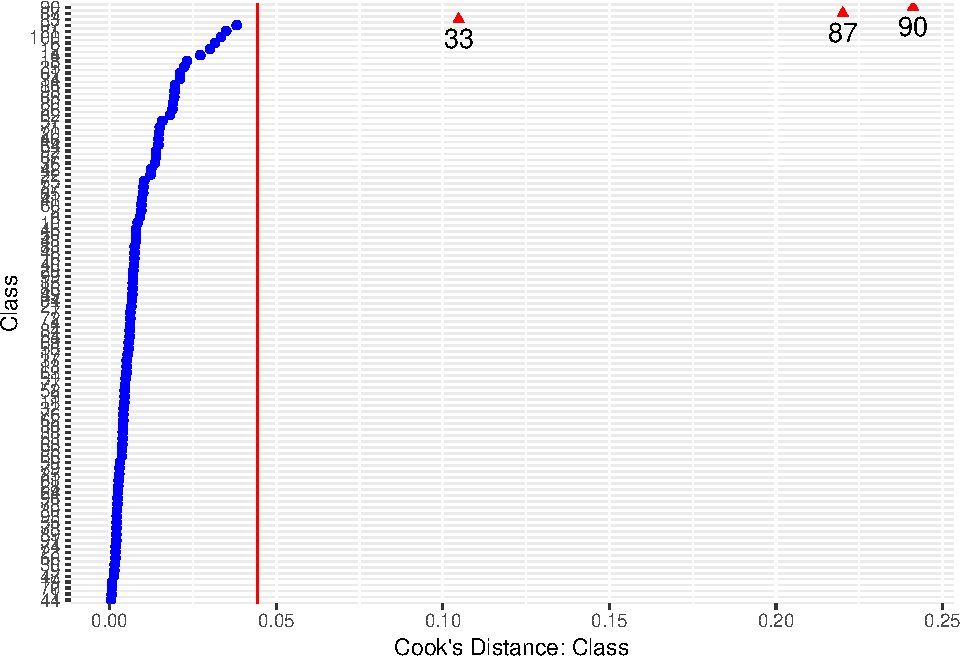
\includegraphics{Beck_HW_5_files/figure-latex/unnamed-chunk-21-1.pdf}

\subsection{Part A}\label{part-a-5}

How many classrooms stand out as distinctly more influential than the
others? 3 classrooms: 33, 87, and 90.

\subsection{Part B}\label{part-b-5}

If those classrooms are excluded from the analysis and the model is
refit, do any conclusions change?

\begin{Shaded}
\begin{Highlighting}[]
\NormalTok{Pop_Fit_}\FloatTok{7.}\NormalTok{cd <-}\StringTok{ }\KeywordTok{update}\NormalTok{(Pop_Fit_}\DecValTok{7}\NormalTok{, }\DataTypeTok{data =}\NormalTok{ dat }\OperatorTok\StringTok{ }\KeywordTok{filter}\NormalTok{(}\OperatorTok{!}\NormalTok{(class }\OperatorTok\StringTok{ }\KeywordTok{c}\NormalTok{(}\DecValTok{87}\NormalTok{, }\DecValTok{33}\NormalTok{, }\DecValTok{90}\NormalTok{))))}

\KeywordTok{table_fun}\NormalTok{(Pop_Fit_}\FloatTok{7.}\NormalTok{cd) }\OperatorTok
\StringTok{  }\KeywordTok{mutate}\NormalTok{(}\DataTypeTok{term =} \KeywordTok{str_replace_all}\NormalTok{(term, }\StringTok{"_"}\NormalTok{, }\StringTok{" "}\NormalTok{)) }\OperatorTok
\StringTok{  }\KeywordTok{select}\NormalTok{(}\OperatorTok{-}\NormalTok{type) }\OperatorTok
\StringTok{  }\KeywordTok{kable}\NormalTok{(., }\StringTok{"latex"}\NormalTok{, }\DataTypeTok{escape =}\NormalTok{ F, }\DataTypeTok{booktabs =}\NormalTok{ T,}
        \DataTypeTok{col.names =} \KeywordTok{c}\NormalTok{(}\StringTok{"Term"}\NormalTok{, }\KeywordTok{c}\NormalTok{(}\StringTok{"b"}\NormalTok{, }\StringTok{"CI"}\NormalTok{))) }\OperatorTok
\StringTok{  }\KeywordTok{add_header_above}\NormalTok{(}\KeywordTok{c}\NormalTok{(}\StringTok{" "}\NormalTok{ =}\StringTok{ }\DecValTok{1}\NormalTok{, }\StringTok{"Fit 7 Outliers Removed"}\NormalTok{)) }\OperatorTok
\StringTok{  }\KeywordTok{group_rows}\NormalTok{(}\StringTok{"Fixed"}\NormalTok{, }\DecValTok{1}\NormalTok{,}\DecValTok{6}\NormalTok{) }\OperatorTok
\StringTok{  }\KeywordTok{group_rows}\NormalTok{(}\StringTok{"Random"}\NormalTok{, }\DecValTok{7}\NormalTok{,}\DecValTok{7}\NormalTok{) }\OperatorTok
\StringTok{  }\KeywordTok{group_rows}\NormalTok{(}\StringTok{"Fixed"}\NormalTok{, }\DecValTok{8}\NormalTok{,}\DecValTok{9}\NormalTok{)}
\end{Highlighting}
\end{Shaded}

\begin{tabular}{lll}
\toprule
\multicolumn{1}{c}{ } & \multicolumn{1}{c}{Fit 7 Outliers Removed} \\
\cmidrule(l{2pt}r{2pt}){2-2}
Term & b & CI\\
\midrule
\addlinespace[0.3em]
\multicolumn{3}{l}{\textbf{Fixed}}\\
\hspace{1em}(Intercept) & 13.17 & [12.00, 14.94]\\
\hspace{1em}extrav & -0.62 & [-0.80, -0.27]\\
\hspace{1em}Mean E GMC & -11.26 & [-13.08, -10.04]\\
\hspace{1em}sexFemale & 0.53 & [-0.24, 0.97]\\
\hspace{1em}extrav:Mean E GMC & 1.08 & [0.73, 1.24]\\
\hspace{1em}Mean E GMC:sexFemale & 0.73 & [0.28, 1.50]\\
\addlinespace[0.3em]
\multicolumn{3}{l}{\textbf{Random}}\\
\hspace{1em}$\tau {00}$ & 0.44 & [0.36, 0.54]\\
$R^2 m$ & 0.43 & \\
$R^2 c$ & 0.68 & \\
\bottomrule
\end{tabular}

No, in terms of significance levels, no conclusions change.


\end{document}
